% GENERATED FILE -- DO NOT EDIT.
%
% Produced by harness/assemble_contract.py from module.yaml and claims/*.tex.
% Edit the claim files and regenerate; `--check` fails if this file is stale.
\documentclass[11pt,a4paper]{article}
\pdftrailerid{c2312062bd916090c8b34d77bc16c7d5}
%% --- 1. Mathematics (order matters: physics after braket wins \ket, \tr) ---
\usepackage{amsmath}
\usepackage{amssymb}
\usepackage{amsfonts}
\usepackage{amsthm}
\usepackage{mathtools}
\usepackage{dsfont}
\usepackage{braket}
\usepackage{physics}
%% --- 2. Page furniture ------------------------------------------------------
\usepackage{xcolor}
\usepackage{array}    % >{...} column prefixes in the wide tables of some claims
\usepackage{enumitem}
\usepackage{graphicx}
\usepackage{booktabs}
\usepackage{longtable}
\usepackage{xltabular}              % front- and back-matter tables across pages
\usepackage{needspace}
\usepackage{xurl}
\usepackage{tcolorbox}
\tcbuselibrary{skins,breakable}
%% --- 3. Links and navigation (hyperref late; bookmark, refcount after it) ---
\usepackage{hyperref}
\usepackage{bookmark}
\usepackage{refcount}
%% --- 4. Colours: every distinction also has a shape (rule, caps, size, weight)
\definecolor{nnGrey}{gray}{0.40}      % non-normative text
\definecolor{metaGrey}{gray}{0.30}    % the generated meta line
\definecolor{techGrey}{gray}{0.45}    % heading of a technical claim
\definecolor{mainRule}{RGB}{0,110,140}
\definecolor{reqAccent}{RGB}{165,70,0}
\definecolor{linkBlue}{RGB}{0,62,150}
\definecolor{extLink}{RGB}{120,40,140}  % links into another PDF
\hypersetup{colorlinks=true, linkcolor=linkBlue, citecolor=linkBlue,
  urlcolor=linkBlue, filecolor=extLink, bookmarksnumbered=true,
  bookmarksopen=true, bookmarksopenlevel=1, pdfdisplaydoctitle=true}
% A link into another PDF (\href to a .pdf, \hyperref{file}..., xr-hyper) is a
% relative URI, <file>#nameddest=<destination>, in the file-link colour:
% browser viewers (Edge, Chrome) ignore hyperref's default GoToR action.
\makeatletter
\renewcommand*{\hyper@linkfile}[3]{% anchor text, file name, destination
  \begingroup
    \ifx\\#3\\\def\CQ@target{#2}\else\def\CQ@target{#2\hyper@hash nameddest=#3}\fi
    \let\@urlcolor\@filecolor
    \hyper@linkurl{#1}{\CQ@target}%
  \endgroup}
\makeatother
%% --- 5. The mapped Unicode set (harness/contract_navigation.py, UNICODE_TEX)
\DeclareUnicodeCharacter{03B1}{\ensuremath{\alpha}}
\DeclareUnicodeCharacter{03B2}{\ensuremath{\beta}}
\DeclareUnicodeCharacter{03B3}{\ensuremath{\gamma}}
\DeclareUnicodeCharacter{03B4}{\ensuremath{\delta}}
\DeclareUnicodeCharacter{03B5}{\ensuremath{\varepsilon}}
\DeclareUnicodeCharacter{03F5}{\ensuremath{\epsilon}}
\DeclareUnicodeCharacter{03B6}{\ensuremath{\zeta}}
\DeclareUnicodeCharacter{03B7}{\ensuremath{\eta}}
\DeclareUnicodeCharacter{03B8}{\ensuremath{\theta}}
\DeclareUnicodeCharacter{03D1}{\ensuremath{\vartheta}}
\DeclareUnicodeCharacter{03B9}{\ensuremath{\iota}}
\DeclareUnicodeCharacter{03BA}{\ensuremath{\kappa}}
\DeclareUnicodeCharacter{03BB}{\ensuremath{\lambda}}
\DeclareUnicodeCharacter{03BC}{\ensuremath{\mu}}
\DeclareUnicodeCharacter{03BD}{\ensuremath{\nu}}
\DeclareUnicodeCharacter{03BE}{\ensuremath{\xi}}
\DeclareUnicodeCharacter{03C0}{\ensuremath{\pi}}
\DeclareUnicodeCharacter{03C1}{\ensuremath{\rho}}
\DeclareUnicodeCharacter{03F1}{\ensuremath{\varrho}}
\DeclareUnicodeCharacter{03C3}{\ensuremath{\sigma}}
\DeclareUnicodeCharacter{03C2}{\ensuremath{\varsigma}}
\DeclareUnicodeCharacter{03C4}{\ensuremath{\tau}}
\DeclareUnicodeCharacter{03C5}{\ensuremath{\upsilon}}
\DeclareUnicodeCharacter{03C6}{\ensuremath{\varphi}}
\DeclareUnicodeCharacter{03D5}{\ensuremath{\phi}}
\DeclareUnicodeCharacter{03C7}{\ensuremath{\chi}}
\DeclareUnicodeCharacter{03C8}{\ensuremath{\psi}}
\DeclareUnicodeCharacter{03C9}{\ensuremath{\omega}}
\DeclareUnicodeCharacter{0393}{\ensuremath{\Gamma}}
\DeclareUnicodeCharacter{0394}{\ensuremath{\Delta}}
\DeclareUnicodeCharacter{0398}{\ensuremath{\Theta}}
\DeclareUnicodeCharacter{039B}{\ensuremath{\Lambda}}
\DeclareUnicodeCharacter{039E}{\ensuremath{\Xi}}
\DeclareUnicodeCharacter{03A0}{\ensuremath{\Pi}}
\DeclareUnicodeCharacter{03A3}{\ensuremath{\Sigma}}
\DeclareUnicodeCharacter{03A5}{\ensuremath{\Upsilon}}
\DeclareUnicodeCharacter{03A6}{\ensuremath{\Phi}}
\DeclareUnicodeCharacter{03A8}{\ensuremath{\Psi}}
\DeclareUnicodeCharacter{03A9}{\ensuremath{\Omega}}
\DeclareUnicodeCharacter{00E1}{\'a}
\DeclareUnicodeCharacter{00E0}{\`a}
\DeclareUnicodeCharacter{00E2}{\^a}
\DeclareUnicodeCharacter{00E4}{\"a}
\DeclareUnicodeCharacter{00E5}{\aa{}}
\DeclareUnicodeCharacter{00E9}{\'e}
\DeclareUnicodeCharacter{00E8}{\`e}
\DeclareUnicodeCharacter{00EA}{\^e}
\DeclareUnicodeCharacter{00EB}{\"e}
\DeclareUnicodeCharacter{00ED}{\'{\i}}
\DeclareUnicodeCharacter{00EF}{\"{\i}}
\DeclareUnicodeCharacter{00F3}{\'o}
\DeclareUnicodeCharacter{00F2}{\`o}
\DeclareUnicodeCharacter{00F4}{\^o}
\DeclareUnicodeCharacter{00F6}{\"o}
\DeclareUnicodeCharacter{00F8}{\o{}}
\DeclareUnicodeCharacter{00FA}{\'u}
\DeclareUnicodeCharacter{00F9}{\`u}
\DeclareUnicodeCharacter{00FB}{\^u}
\DeclareUnicodeCharacter{00FC}{\"u}
\DeclareUnicodeCharacter{00F1}{\~n}
\DeclareUnicodeCharacter{00E7}{\c{c}}
\DeclareUnicodeCharacter{00DF}{\ss{}}
\DeclareUnicodeCharacter{00C4}{\"A}
\DeclareUnicodeCharacter{00C5}{\AA{}}
\DeclareUnicodeCharacter{00C9}{\'E}
\DeclareUnicodeCharacter{00D6}{\"O}
\DeclareUnicodeCharacter{00DC}{\"U}
\DeclareUnicodeCharacter{2013}{\textendash{}}
\DeclareUnicodeCharacter{2014}{\textemdash{}}
\DeclareUnicodeCharacter{2018}{`}
\DeclareUnicodeCharacter{2019}{'}
\DeclareUnicodeCharacter{201C}{``}
\DeclareUnicodeCharacter{201D}{''}
\DeclareUnicodeCharacter{2026}{\ldots{}}
\DeclareUnicodeCharacter{00A0}{~}
\DeclareUnicodeCharacter{00A7}{\S{}}
\DeclareUnicodeCharacter{2264}{\ensuremath{\le}}
\DeclareUnicodeCharacter{2265}{\ensuremath{\ge}}
\DeclareUnicodeCharacter{2260}{\ensuremath{\neq}}
\DeclareUnicodeCharacter{2248}{\ensuremath{\approx}}
\DeclareUnicodeCharacter{2261}{\ensuremath{\equiv}}
\DeclareUnicodeCharacter{223C}{\ensuremath{\sim}}
\DeclareUnicodeCharacter{2243}{\ensuremath{\simeq}}
\DeclareUnicodeCharacter{2245}{\ensuremath{\cong}}
\DeclareUnicodeCharacter{221D}{\ensuremath{\propto}}
\DeclareUnicodeCharacter{226A}{\ensuremath{\ll}}
\DeclareUnicodeCharacter{226B}{\ensuremath{\gg}}
\DeclareUnicodeCharacter{2192}{\ensuremath{\to}}
\DeclareUnicodeCharacter{2190}{\ensuremath{\leftarrow}}
\DeclareUnicodeCharacter{2194}{\ensuremath{\leftrightarrow}}
\DeclareUnicodeCharacter{21D2}{\ensuremath{\Rightarrow}}
\DeclareUnicodeCharacter{21D0}{\ensuremath{\Leftarrow}}
\DeclareUnicodeCharacter{21D4}{\ensuremath{\Leftrightarrow}}
\DeclareUnicodeCharacter{21A6}{\ensuremath{\mapsto}}
\DeclareUnicodeCharacter{2208}{\ensuremath{\in}}
\DeclareUnicodeCharacter{2209}{\ensuremath{\notin}}
\DeclareUnicodeCharacter{2286}{\ensuremath{\subseteq}}
\DeclareUnicodeCharacter{2282}{\ensuremath{\subset}}
\DeclareUnicodeCharacter{2287}{\ensuremath{\supseteq}}
\DeclareUnicodeCharacter{2283}{\ensuremath{\supset}}
\DeclareUnicodeCharacter{2229}{\ensuremath{\cap}}
\DeclareUnicodeCharacter{222A}{\ensuremath{\cup}}
\DeclareUnicodeCharacter{2216}{\ensuremath{\setminus}}
\DeclareUnicodeCharacter{2205}{\ensuremath{\emptyset}}
\DeclareUnicodeCharacter{2200}{\ensuremath{\forall}}
\DeclareUnicodeCharacter{2203}{\ensuremath{\exists}}
\DeclareUnicodeCharacter{2115}{\ensuremath{\mathbb{N}}}
\DeclareUnicodeCharacter{2124}{\ensuremath{\mathbb{Z}}}
\DeclareUnicodeCharacter{211A}{\ensuremath{\mathbb{Q}}}
\DeclareUnicodeCharacter{211D}{\ensuremath{\mathbb{R}}}
\DeclareUnicodeCharacter{2102}{\ensuremath{\mathbb{C}}}
\DeclareUnicodeCharacter{00B7}{\ensuremath{\cdot}}
\DeclareUnicodeCharacter{00D7}{\ensuremath{\times}}
\DeclareUnicodeCharacter{2212}{\ensuremath{-}}
\DeclareUnicodeCharacter{00B1}{\ensuremath{\pm}}
\DeclareUnicodeCharacter{2213}{\ensuremath{\mp}}
\DeclareUnicodeCharacter{221A}{\ensuremath{\surd}}
\DeclareUnicodeCharacter{2211}{\ensuremath{\sum}}
\DeclareUnicodeCharacter{220F}{\ensuremath{\prod}}
\DeclareUnicodeCharacter{222B}{\ensuremath{\int}}
\DeclareUnicodeCharacter{221E}{\ensuremath{\infty}}
\DeclareUnicodeCharacter{2202}{\ensuremath{\partial}}
\DeclareUnicodeCharacter{2207}{\ensuremath{\nabla}}
\DeclareUnicodeCharacter{2297}{\ensuremath{\otimes}}
\DeclareUnicodeCharacter{2295}{\ensuremath{\oplus}}
\DeclareUnicodeCharacter{2218}{\ensuremath{\circ}}
\DeclareUnicodeCharacter{2308}{\ensuremath{\lceil}}
\DeclareUnicodeCharacter{2309}{\ensuremath{\rceil}}
\DeclareUnicodeCharacter{230A}{\ensuremath{\lfloor}}
\DeclareUnicodeCharacter{230B}{\ensuremath{\rfloor}}
\DeclareUnicodeCharacter{27E8}{\ensuremath{\langle}}
\DeclareUnicodeCharacter{27E9}{\ensuremath{\rangle}}
\DeclareUnicodeCharacter{2016}{\ensuremath{\|}}
\DeclareUnicodeCharacter{2113}{\ensuremath{\ell}}
\DeclareUnicodeCharacter{00B0}{\ensuremath{^{\circ}}}
\DeclareUnicodeCharacter{00B2}{\ensuremath{^{2}}}
\DeclareUnicodeCharacter{00B3}{\ensuremath{^{3}}}
\DeclareUnicodeCharacter{00B9}{\ensuremath{^{1}}}
\DeclareUnicodeCharacter{2080}{\ensuremath{_{0}}}
\DeclareUnicodeCharacter{2081}{\ensuremath{_{1}}}
\DeclareUnicodeCharacter{2082}{\ensuremath{_{2}}}
\DeclareUnicodeCharacter{207F}{\ensuremath{^{n}}}
\DeclareUnicodeCharacter{2096}{\ensuremath{_{k}}}
%% --- 6. Numbering: one counter per section -----------------------
\numberwithin{equation}{section}
\setcounter{tocdepth}{1}
%% --- 7. The project macro set, then the claim environments -----------------
% spec/macros.tex, read relative to this module's directory (latexmk -cd).
% =============================================================================
%  spec/macros.tex -- the one macro set every generated contract inputs.
%
%  Two parts: part A, the macros spec/notation.md catalogues, and part B,
%  the macros local to one module, grouped by module.
%  harness/assemble_contract.py emits \input{../../macros} for it, so the
%  file is read from spec/modules/<id>/.
%
%  RULES
%    * A macro that spec/notation.md catalogues is a verbatim copy of it
%      (part A). Changing one is a notation change: bump spec/notation.md.
%    * Part B holds the module-local macros. A macro defined by two modules
%      with the same expansion appears once, under the first module (in the
%      order below) that defines it. Two macros with the same name and
%      DIFFERENT expansions are both kept under a module prefix, and the
%      claims write the prefixed names:
%        \Chain  -> \redChain (reductions, \mathfrak{C}: the reduction chain)
%                   \pcChain  (protocol-compiler, \mathfrak{R}: the two-segment
%                             chain; \Chsrc and \Chrec are built on it)
%        \Nmsm   -> \redNmsm  (reductions, \mathcal{N}: a POVM measurement
%                             channel)
%                   \pcNmsm   (\mathcal{N}_{\mathsf A}: Alice's measurement
%                             channel, written by
%                             transmitter/thm:certificate-sufficiency,
%                             transmitter/rem:xreg and
%                             reductions/lem:source-transfer)
%    * Deliberately omitted: a \provenance{tag}{details} macro. Provenance
%      is a header field of every claim file (spec/claim-format.md section
%      3); a claim body that calls such a macro fails to compile, which is
%      the intended signal.
%
%  REQUIRED PACKAGES, loaded by the assembler's preamble before this file:
%    amsmath, amssymb, amsfonts, mathtools, dsfont, braket, physics, xcolor
%    (braket before physics, so that physics wins for \ket, \bra, \tr, ...).
%
%  This file contains only definitions: no \usepackage, no document body.
% =============================================================================


% =============================================================================
%  PART A -- notation macros, the ones spec/notation.md catalogues, each a
%  verbatim copy of its catalogue row; grouped under numbered headings.
% =============================================================================

% -----------------------------------------------------------------------------
% 1. State spaces and operator sets (a "system label" -> spaces of operators)
% -----------------------------------------------------------------------------
\newcommand{\Hs}[1]{\mathcal{H}(#1)}        % Hilbert space of a system label
\newcommand{\Lin}[1]{\mathcal{L}(#1)}       % bounded linear operators on H(#1)
\newcommand{\Linn}[2]{\mathcal{L}(#1,#2)}   % linear maps H(#1) -> H(#2)
\newcommand{\Pos}[1]{\mathrm{Pos}(#1)}      % positive semidefinite operators on H(#1)
\newcommand{\Density}{\mathrm{D}}           % density operators: \Density(A) = D(A)
\newcommand{\Seq}[1]{S_{=}(#1)}             % normalized states (trace = 1)
\newcommand{\Sleq}[1]{S_{\leq}(#1)}         % subnormalized states (0 <= trace <= 1)
\newcommand{\id}{\mathds{1}}                % identity operator
\newcommand{\idon}[1]{\mathds{1}_{#1}}      % identity on a named system, e.g. \idon{C}

% DEPRECATED: applies \mathcal to both arguments itself, so it takes bare
% letters, not system labels. Prefer \Linn; do not use in new contracts.
\providecommand{\Lop}[2]{\mathcal{L}(\mathcal{#1}, \mathcal{#2})}


% -----------------------------------------------------------------------------
% 2. Composite systems
% -----------------------------------------------------------------------------
\newcommand{\dsum}{\oplus}                  % direct sum of system labels
% Tensor product: use \otimes directly.
% n-fold direct sum of an operator space: \Lin{A}^{\oplus n}


% -----------------------------------------------------------------------------
% 3. Events, conditioning and classical registers (for STATES)
%    Convention:  \wedge  -> subnormalized "and-event" component, e.g. \rho_{A\wedge x}
%                 |        -> normalized conditional state,        e.g. \rho_{A|x}
% (Write these directly in subscripts; no extra macros needed.)
% -----------------------------------------------------------------------------


% -----------------------------------------------------------------------------
% 4. Photon-number subspaces / direct-sum blocks
%    Convention:  operators carry the restriction "on top", in brackets;
%                 states carry it as a \wedge subscript (see Sec. 3).
% -----------------------------------------------------------------------------
\newcommand{\Pnum}[1]{P_{#1}}               % photon-number projector (system from context)
\newcommand{\Pnumon}[2]{P_{#1}^{#2}}        % with explicit system superscript, e.g. P_n^C
\newcommand{\blk}[2]{#1^{(#2)}}             % operator block, e.g. \blk{M}{\leqN} = M^{(<=N)}
\newcommand{\leqN}{\leq N}                  % use as \blk{M}{\leqN}
\newcommand{\gtN}{> N}                      % use as \blk{M}{\gtN}
\newcommand{\eqn}{= n}                      % use as \blk{M}{\eqn}


% -----------------------------------------------------------------------------
% 5. System labels used in the protocol
% -----------------------------------------------------------------------------
\newcommand{\Chan}{C}                       % quantum-channel (Eve) input to Bob
\newcommand{\Prb}{P}                        % probe input
\newcommand{\Flag}{{\mathrm{Flg}}}          % flag system (EXISTS ONLY AFTER squashing)
\newcommand{\Loss}{{\mathrm{Lss}}}          % loss system
\newcommand{\Vc}{{\mathrm{Vcm}}}            % vacuum system
\newcommand{\Nout}{N_{\mathrm{out}}}
\newcommand{\Nin}{N_{\mathrm{in}}}


% -----------------------------------------------------------------------------
% 6. Alphabets
% -----------------------------------------------------------------------------
\newcommand{\Yset}{\mathcal{Y}}             % Bob's (coarse-grained) detection alphabet
\newcommand{\Yraw}{\mathcal{Y}_{\mathrm{raw}}}% raw click patterns {0,1}^4
\newcommand{\Yscset}{\mathcal{Y}_{\singlec}}% single-click outcomes
\newcommand{\Ymcset}{\mathcal{Y}_{\mc}}     % multi-click outcomes
\newcommand{\Tset}{\mathcal{T}_{\mathrm{set}}}% private setting set (the probe settings in the optical instance)
\newcommand{\Xset}{\mathcal{X}}             % Alice's alphabet
\newcommand{\Dset}{\{H,V,+,-\}}             % polarization / detector labels
\newcommand{\pass}{\top}                    % pass sifting


% -----------------------------------------------------------------------------
% 7. Mode / outcome abbreviations
% -----------------------------------------------------------------------------
\newcommand{\on}{{\mathrm{on}}}
\newcommand{\off}{{\mathrm{off}}}
\newcommand{\dc}{{\mathrm{dc}}}             % dark count
\newcommand{\sq}{\mathrm{sq}}               % squashed
\newcommand{\mc}{\mathrm{mc}}               % multi-click
\newcommand{\nc}{\mathrm{nc}}               % no-click
\newcommand{\singlec}{\mathrm{sc}}          % single-click
\newcommand{\vac}{\mathrm{vac}}             % vacuum
\newcommand{\kout}{{k_\mathrm{out}}}
\newcommand{\kin}{{k_\mathrm{in}}}


% -----------------------------------------------------------------------------
% 8. Maps, channels and miscellaneous operators
% -----------------------------------------------------------------------------
\newcommand{\Prob}{\mathrm{Prob}}           % probability (use \Prob[\cdot] or \Prob(\cdot))
\newcommand{\lmin}{\lambda_{\min}}          % minimum eigenvalue
\newcommand{\Wflag}{W_{\Flag}}              % flag-space weight
\newcommand{\transpose}{\mathsf{T}}
\newcommand{\innerp}[2]{\left\langle #1 \vert #2 \right\rangle}
\renewcommand{\vec}[1]{\boldsymbol{#1}}     % NB: overrides the LaTeX arrow accent


% -----------------------------------------------------------------------------
% 9. Key-rate numerics
% -----------------------------------------------------------------------------
\newcommand{\cG}{\mathcal{G}}               % protocol map
\newcommand{\cZ}{\mathcal{Z}}               % pinching map
\newcommand{\Amap}{\mathcal{A}_{\mathrm{ann}}} % announcement + measurement map
\newcommand{\Amapnb}{\mathcal{A}_{\mathrm{ann}|\mathrm{nb}}}
\newcommand{\simpl}{}                       % empty suffix for simplified block maps
\newcommand{\acSet}{\mathcal{S}_{\mathrm{acc}}} % acceptance set
\newcommand{\testE}{\mathcal{E}_{\mathrm{test}}} % test-statistics map
\newcommand{\ecLeak}{\mathrm{leak}^{\mathrm{EC}}_{\mathrm{obs}}}
\newcommand{\pgen}{p_{\mathrm{gen}}}
\newcommand{\askeyr}{R_{\infty}}             % asymptotic key rate
\newcommand{\ppass}{p_{\mathrm{pass}}}       % sifting pass probability


% -----------------------------------------------------------------------------
% 10. Finite-size analysis / Renyi entropies
% -----------------------------------------------------------------------------

% --- Round types: test vs. key generation (register T, alphabet \Fset) --------
\newcommand{\tst}{\mathrm{test}}            % test round
\newcommand{\gen}{\mathrm{gen}}             % key-generation round
\newcommand{\Fset}{\mathcal{T}}             % round-type alphabet {test, gen} (not \Tset)
\newcommand{\Chat}{\widehat{C}}             % acceptance-test register
\newcommand{\Chatset}{\widehat{\mathcal{C}}}% its alphabet

% --- Basis / key extraction functions ----------------------------------------
\newcommand{\bA}{b_{A}}                     % Alice's basis-extraction function
\newcommand{\bB}{b_{B}}                     % Bob's basis-extraction function
\newcommand{\kB}{k_{B}}                     % Bob's key-extraction function

% --- Maps --------------------------------------------------------------------
\newcommand{\Mprot}{\mathcal{M}}            % single-round protocol map
\newcommand{\Phimap}{\boldsymbol{\Phi}}     % test-statistics map
\newcommand{\Pdeph}{\mathcal{P}}            % dephasing (pinching) map on \Blreg

% --- Isometries --------------------------------------------------------------
\newcommand{\Vmsm}{V_{\mathrm{msm}}}        % measurement isometry
\newcommand{\Vann}{V_{\mathrm{ann}}}        % announcement isometry
\newcommand{\VI}{V_{I}}                     % Eve's copy of the announcements
\newcommand{\VChat}{V_{\Chat}}              % acceptance-data isometry
\newcommand{\VR}{V_{R}}                     % sifting + key map -> raw key R
\newcommand{\VZ}{V_{Z}}                     % raw key -> key register Z
\newcommand{\Wprot}{W}                      % full protocol isometry

% --- Renyi entropies ---------------------------------------------------------
% SECURITY-CRITICAL: see spec/notation.md §4. Never change an arrow to
% make an inequality work out; never convert silently between the sandwiched
% (tilde) and Petz (overline) families.
\newcommand{\Hsandup}{\widetilde{H}^{\uparrow}_{\alpha}}   % sandwiched, up
\newcommand{\Hsanddown}{\widetilde{H}^{\downarrow}_{\alpha}}% sandwiched, down
\newcommand{\Hpetzup}{\overline{H}^{\uparrow}_{\alpha}}    % Petz, up
\newcommand{\Hpetzdown}{\overline{H}^{\downarrow}_{\alpha}}% Petz, down
\newcommand{\hup}{h^{\uparrow}_{\alpha}}                   % single-round rate
\newcommand{\hqkd}{h^{\uparrow,\mathrm{QKD}}_{\alpha}}     % single-round QKD rate
\newcommand{\hlow}{\underline{h}_{\alpha}}                 % lower bound on \hqkd
% --- spec/notation.md 3.5 and 4.5 -------------------------------------------
% \hlb  is the first-order linearization lower bound on \hlow: the headline
%       key rate (the `first-order` tier of foundations/def:tiers). NOT \hlow
%       itself.
% \tnum is the instance's one declared numerical tolerance. Its
%       near-collision with the declared marginal \tau_A is disclosed in
%       spec/notation.md 3.5; bare \tau is reserved and denotes neither.
\newcommand{\hlb}{\underline{h}^{\mathrm{FO}}_{\alpha}}    % first-order lower bound on \hlow
\newcommand{\tnum}{\tau_{\mathrm{num}}}                    % declared numerical tolerance


% =============================================================================
%  PART B -- module-local macros, grouped by module. Deprecated aliases,
%  defined so that a text written with them compiles, used in no new contract: \Lop,
%  \testE, \Pdeph, \pass, \ecLeak (spec/notation.md section 3.9).
% =============================================================================

% --- meat-core -----------------------------------------------------------------
\newcommand{\SecSet}{\mathbb{S}}            % sector index set of Q
\newcommand{\Qsys}{Q}                       % declared sector-carrying measured system
\newcommand{\Vset}{\mathcal{V}}             % declared joint outcome alphabet of the Q-POVM
\newcommand{\CAset}{\mathcal{C}_{A}}        % Alice announcement alphabet
\newcommand{\CBset}{\mathcal{C}_{B}}        % Bob announcement alphabet
\newcommand{\Party}{\mathfrak{P}}           % declared party partition
\newcommand{\Oset}[1]{\mathcal{O}_{#1}}     % readout alphabet of party #1
\newcommand{\rd}[1]{\pi_{#1}}               % readout map of party #1
\newcommand{\Sadm}{\mathcal{S}_{A}}         % admissible Alice subspace
\newcommand{\nomarg}{\mathsf{none}}         % "no trusted marginal declared"
\newcommand{\Zset}{\mathcal{Z}_{\perp}}     % raw-key alphabet incl. \perp
\newcommand{\Zval}{\mathcal{Z}}             % key alphabet without \perp
\newcommand{\Etil}{\widetilde{E}}           % single-round purifying register
\newcommand{\Ehat}{\widehat{E}}             % Eve's n-round register
\newcommand{\OmAT}{\Omega_{\mathrm{AT}}}    % acceptance event
\newcommand{\epa}{\varepsilon_{\mathrm{PA}}}
\newcommand{\eev}{\varepsilon_{\mathrm{EV}}}
\newcommand{\lEC}{\lambda_{\mathrm{EC}}}
\newcommand{\Decl}{\mathfrak{D}}            % protocol declaration
\newcommand{\CList}{\mathfrak{L}}           % declared constraint list
\newcommand{\PinS}{\mathcal{P}_{\SecSet}}   % sector pinching on Q
\newcommand{\Feas}{\mathcal{W}}             % feasible set of block states
\newcommand{\Chkey}{\Chatset_{\mathrm{key}}}% key-live acceptance values
\newcommand{\Kann}{\mathcal{K}}             % announcement-class alphabet
\newcommand{\hold}{\mathsf{h}}              % declared key holder (A or B)
\newcommand{\sfD}{D}                        % classical KL divergence (base 2)
\newcommand{\Dtwo}{D}                       % quantum relative entropy (base 2)
\newcommand{\Dsand}{\widetilde{D}_{\alpha}} % sandwiched Renyi divergence
\newcommand{\idmap}{\mathrm{id}}            % identity channel
\newcommand{\Aev}{\mathcal{A}}              % Eve's per-round attack channel
\newcommand{\AttSet}{\mathfrak{A}}          % licensed attack-channel set
\newcommand{\Chacc}{\Chatset_{\mathrm{acc}}}% acceptance support of \acSet
\newcommand{\epsstar}{\varepsilon^{\star}}      % distance to an exact POVM
\newcommand{\dfH}{\Delta_{\mathrm{herm}}}       % Hermiticity defect
\newcommand{\dfP}{\Delta_{\mathrm{pos}}}        % negative part
\newcommand{\dfC}{\Delta_{\mathrm{cpl}}}        % completeness defect
\newcommand{\lmoq}{g}                       % acceptance-side gradient block
\newcommand{\lmoJ}{G}                       % feasible-side gradient block
\newcommand{\bacc}{\beta_{\mathrm{acc}}}    % certified acceptance-side minimum
\newcommand{\Itset}{\mathfrak{I}}           % finite index set of iterates (C22)

% --- reductions ----------------------------------------------------------------
\newcommand{\Bsys}{B}                        % physical (pre-squashing) system
\newcommand{\Tcl}[1]{\mathcal{T}(#1)}        % trace-class operators on H(#1)
\newcommand{\Ins}{\mathcal{I}}               % generalized-instrument branch map
\newcommand{\redNmsm}{\mathcal{N}}              % POVM measurement channel
\newcommand{\Eprot}{\mathcal{E}}             % n-round protocol channel
\newcommand{\Grnd}{\mathsf{G}}               % one round map of a protocol
\newcommand{\Kfin}{\mathsf{K}}               % end-of-protocol processing
\newcommand{\Crit}{\mathsf{sec}}             % value of a security criterion
\newcommand{\Pflag}{\Pi_{\Flag}}             % flag-sector projector on Q
\newcommand{\Pleq}{\Pi_{\leqN}}              % preserved-block projector
\newcommand{\Pgt}{\Pi_{\gtN}}                % above-cutoff projector
\newcommand{\Sph}{S^{\mathrm{ph}}}           % family of physical inputs
\newcommand{\Srch}{S^{\mathrm{rch}}}         % reachable squashed states
\newcommand{\Ssq}{S^{\sq}}                   % squashed admissible set
\newcommand{\Ffss}{F^{\mathrm{FSS}}}         % flag-state-squasher target
\newcommand{\Fwp}{F^{\mathrm{WP}}}           % multi-bound WPFSS target
\newcommand{\Mwp}{M^{\mathrm{WP}}}           % renormalized above-cutoff POVM
\newcommand{\Mdec}{{M'}^{\mathrm{ph}}}       % declared physical family on B
\newcommand{\Ppvm}{P^{\Flag}}                % flag PVM
\newcommand{\Lmp}{{\Lambda_{\mathrm{mp}}}}   % measure-and-prepare channel
\newcommand{\Lwp}{{\Lambda^{\mathrm{WP}}}}   % multi-bound WPFSS channel
\newcommand{\Lfss}{{\Lambda^{\mathrm{FSS}}}} % flag-state-squasher channel
\newcommand{\lmax}{\lambda_{\max}}           % maximum eigenvalue
\newcommand{\Lnoise}{\widetilde{\Lambda}}    % flag-noise channel
\newcommand{\cg}{\varpi}                     % declared coarse-graining map
\newcommand{\MCK}{\mathsf{MC}}               % multiclick raw-pattern set
\newcommand{\redChain}{\mathfrak{C}}            % reduction chain
\newcommand{\Lnk}{\ell}                      % a single typed link
\newcommand{\dsq}{\preceq}                      % the squashing relation
\newcommand{\opn}[1]{\left\lVert #1\right\rVert}           % operator (spectral) norm
\newcommand{\mxn}[1]{\left\lVert #1\right\rVert_{\max}}    % entrywise max modulus
\newcommand{\Fld}{\mathbb{F}}                   % exact ordered substrate field
\newcommand{\Fldi}{\mathbb{F}_{i}}              % its Gaussian extension F + iF
\newcommand{\lat}[1]{\big\lfloor #1\big\rfloor_{\kappa}} % round DOWN onto the lattice

% --- protocol-compiler ---------------------------------------------------------
\newcommand{\Spec}{\mathfrak{S}}             % protocol specification (compiler input)
\newcommand{\pcChain}{\mathfrak{R}}            % reduction chain (two typed segments)
\newcommand{\Chsrc}{\pcChain_{\mathrm{src}}}   % its Alice-side source-map segment
\newcommand{\Chrec}{\pcChain_{\mathrm{rec}}}   % its receiver-side squashing segment
\newcommand{\rvirt}{\rho^{\mathrm{v}}}       % virtual (PRE-source-map) signal state
\newcommand{\Fph}{F^{\mathrm{ph}}}           % physical (pre-reduction) POVM element
\newcommand{\Vph}{\mathcal{V}^{\mathrm{ph}}} % physical outcome alphabet
\newcommand{\Tpub}{\mathcal{T}_{\mathrm{pub}}}% public-choice alphabet
\newcommand{\Uset}{\mathcal{U}}              % residual outcome alphabet
\newcommand{\idxm}{\mathsf{idx}}             % label-to-index map
\newcommand{\Asig}{A'}                       % transmitted (signal) system -- the REAL one
\newcommand{\Avirt}{A''}                     % virtual transmitted system (source descriptor of Xi_1)
\newcommand{\Abar}{\bar{A}}                  % Alice's measured register
\newcommand{\Ahat}{\hat{A}}                  % Alice's shield register
\newcommand{\pcNmsm}{\mathcal{N}_{\mathsf A}}  % Alice's measurement channel (see the RULES block)
\newcommand{\Phip}{\Phi^{+}}                 % maximally entangled vector label
\newcommand{\Smap}{\mathfrak{s}}             % the emitted sector map (fraktur: a compile-time object)

% --- receiver ------------------------------------------------------------------
\newcommand{\Modes}{\mathbb{M}}              % declared ordered mode set
\newcommand{\Inp}{\mathbb{I}}                % declared input modes
\newcommand{\InpC}{\mathbb{I}_{\Chan}}       % channel input modes
\newcommand{\InpS}{\mathbb{I}_{\Prb}}        % probe (source) input modes
\newcommand{\Env}{\mathbb{E}}                % dilation (environment) modes
\newcommand{\Port}[1]{\mathbb{P}_{#1}}       % mode set of detector port #1
\newcommand{\Emd}[1]{E_{#1}}                 % coordinate projector on modes #1
\newcommand{\Gmat}{G}                        % instrument (transfer) matrix
\newcommand{\Fock}{\mathfrak{F}}             % Fock / second-quantization functor
\newcommand{\Symn}[1]{\mathrm{Sym}^{#1}}     % symmetric tensor power
\newcommand{\normord}[1]{{:}\mspace{2mu}#1\mspace{2mu}{:}}   % normal ordering
\newcommand{\rk}{\operatorname{rank}}        % rank (physics.sty owns \rank)
\newcommand{\SCK}{\mathsf{SC}}               % single-click pattern set
\newcommand{\Recv}{\mathfrak{R}}             % receiver instrument tuple
\newcommand{\Cat}{\mathfrak{C}}              % component catalogue
\newcommand{\Grph}{\mathfrak{E}}             % declared element graph
\newcommand{\defic}{\mathbb{L}}              % loss deficiency operator
\newcommand{\Pvac}[1]{\Pi_{\vac}(#1)}        % joint no-click element on ports #1
\newcommand{\pmc}{p_{\mc}}                   % uniform high-photon mc weight
\newcommand{\Bnd}{\beta}                     % the scalar bound function beta(n)
\newcommand{\Rot}{R}                         % planar rotation matrix
\newcommand{\Wplate}{W}                      % retarder (wave-plate) matrix
\newcommand{\Bsp}{B}                         % beamsplitter core matrix

% --- statistics ----------------------------------------------------------------
\newcommand{\honest}{p^{\mathrm{hon}}}          % honest per-round distribution
\newcommand{\ecomp}{\varepsilon_{\mathrm{comp}}}% completeness budget
\newcommand{\simplex}[1]{\Delta(#1)}            % probability simplex
\newcommand{\Chatcon}{\Chatset_{\mathrm{con}}}  % constrained outcomes
\newcommand{\Ireg}[3]{\mathcal{I}_{#1}(#2,#3)}  % regularized incomplete beta
\newcommand{\Ncount}[1]{\mathsf{N}_{#1}}        % per-outcome count
\newcommand{\qlo}{\mathbf{q}^{-}}               % box lower bounds
\newcommand{\qhi}{\mathbf{q}^{+}}               % box upper bounds

\makeatletter
\newcommand*{\ClaimHeadFont}{\bfseries}   % switched by prominence
\newcommand*{\ClaimNoteFont}{\mdseries}
\newcommand*{\ClaimShortId}{}
\newcommand*{\SetShortId}[1]{\renewcommand*{\ClaimShortId}{#1}}
\newcommand*{\RestatedName}{}
% Upright bodies throughout: italic is reserved for non-normative text.
% \@endparpenalty\@M keeps the meta line on the statement's page.
\newtheoremstyle{claim}{\topsep}{\topsep}{\normalfont\@endparpenalty\@M}{}%
  {\ClaimHeadFont}{.}{.5em}{\thmname{#1}\thmnumber{ #2}\thmnote{ {\ClaimNoteFont(#3)}}}
\newtheoremstyle{claimass}{\topsep}{\topsep}{\normalfont\@endparpenalty\@M}{}%
  {\ClaimHeadFont}{.}{.5em}{\thmname{#1}\thmnumber{ #2}%
  \ifx\ClaimShortId\@empty\else\ [\textsf{\ClaimShortId}]\fi%
  \thmnote{ {\ClaimNoteFont(#3)}}}
\newtheoremstyle{claimremark}{.5\topsep}{.5\topsep}{\small\@endparpenalty\@M}{}%
  {\itshape}{.}{.5em}{\thmname{#1}\thmnumber{ #2}\thmnote{ {\upshape(#3)}}}
\newtheoremstyle{claimreq}{\topsep}{\topsep}{\normalfont\@endparpenalty\@M}{}%
  {\color{reqAccent}\scshape}{.}{.5em}%
  {\thmname{#1}\thmnumber{ #2}\thmnote{ {\upshape(#3)}}}
\makeatother
\theoremstyle{claim}
\newtheorem{theorem}{Theorem}[section]
\newtheorem{lemma}[theorem]{Lemma}
\newtheorem{proposition}[theorem]{Proposition}
\newtheorem{corollary}[theorem]{Corollary}
\newtheorem{fact}[theorem]{Fact}
\newtheorem{definition}[theorem]{Definition}
\newtheorem*{restatedclaim}{\RestatedName}
\theoremstyle{claimass}
\newtheorem{assumption}[theorem]{Assumption}
\newtheorem*{restatedassumption}{\RestatedName}
\theoremstyle{claimremark}
\newtheorem{remark}[theorem]{Remark}
\newtheorem{example}[theorem]{Example}
\theoremstyle{claimreq}
\newtheorem{requirement}[theorem]{Requirement}
\newtheorem*{restatedrequirement}{\RestatedName}
%% --- 8. Prominence: main results a margin rule and a bold heading ----------
\newtcolorbox{mainclaim}{enhanced jigsaw, breakable, blanker,
  borderline west={1.5pt}{-8pt}{mainRule}, left=0pt, right=0pt, top=0pt, bottom=0pt,
  boxsep=0pt, before skip=\topsep, after skip=\topsep, parbox=false,
  before upper={\renewcommand*{\ClaimNoteFont}{\bfseries}}}
\newenvironment{technicalclaim}{\renewcommand*{\ClaimHeadFont}{\mdseries\color{techGrey}}%
  \renewcommand*{\ClaimNoteFont}{}}{}
%% --- 9. Non-normative text, the meta line, navigation ------------------------
\makeatletter
% Tie what follows to this paragraph: no page break, no list penalty before
% the next theorem head (the \@nobreak route a section heading uses).
\newcommand{\keepwithnext}{\par\nobreak\vspace{3pt}\@nobreaktrue
  \everypar{\if@nobreak\@nobreakfalse\clubpenalty\@M\else\clubpenalty\@clubpenalty\everypar{}\fi}}
\newcommand{\claimsummary}[2]{% #1 claim id (named destination), #2 summary
  \par\addvspace{\bigskipamount}\Needspace{6\baselineskip}%
  {\small\itshape\color{nnGrey}\noindent\hypertarget{claim-#1}{}#2\par}\keepwithnext}
\newcommand{\claimanchor}[1]{% a claim without a summary: the destination alone
  \par\addvspace{\bigskipamount}\Needspace{6\baselineskip}%
  \phantomsection\hypertarget{claim-#1}{}\keepwithnext}
\newcommand{\claimleadin}[1]{{\color{nnGrey}\noindent#1\par}\keepwithnext}
\newcommand{\claimmeta}[1]{\par\nobreak\vspace{2pt}%
  {\footnotesize\color{metaGrey}\raggedright\interlinepenalty\@M\noindent#1\par}%
  \addvspace{\medskipamount}}
% After an assumption: the sentence generated from its verification field; after
% any claim with one: its plain-text reading (user_statement). Both
% non-normative, both grey.
\newcommand{\claimverification}[1]{\par\nobreak\vspace{2pt}%
  {\footnotesize\color{metaGrey}\noindent#1\par}\nobreak}
\newcommand{\claimreading}[1]{\par\nobreak\vspace{2pt}%
  {\footnotesize\color{nnGrey}\noindent\emph{Reading:}\enspace#1\par}\nobreak}
\makeatother
\newcommand{\claimbookmark}[4]{% #1 id, #2 kind word, #3 label, #4 plain title
  \bookmark[dest=claim-#1,level=2]{#2 \getrefnumber{#3} #4}}
\newcommand{\metasep}{\unskip\enspace\textperiodcentered\enspace\ignorespaces}
\newcommand{\metalabel}[1]{\emph{#1}\enspace}
\newcommand{\sectionintro}[1]{{\color{nnGrey}\noindent#1\par}\smallskip}
\newcommand{\sectionimports}[1]{{\footnotesize\color{metaGrey}\raggedright\noindent\metalabel{Imports}#1\par}\smallskip}
\newenvironment{overview}{\par\color{nnGrey}\itshape\noindent\ignorespaces}{\par}
% References: the whole "Def. 2.1" is the link; ids are the fallback text of
% every link into another PDF (a relative URI to a named destination).
\newcommand{\mref}[2]{\hyperref[#2]{#1~\ref*{#2}}}
\newcommand{\aref}[2]{\hyperref[#2]{\textsf{#1}}}
\DeclareUrlCommand{\claimid}{\urlstyle{sf}\def\UrlBreaks{\do\/\do\:\do\-\do\.\do\_}%
  \def\UrlBigBreaks{}\def\UrlNoBreaks{}}
\newcommand{\extref}[2]{\hyperref{#1}{}{claim-#2}{\claimid{#2}}}
\newcommand{\extaref}[3]{\hyperref{#1}{}{claim-#2}{\textsf{#3}}}
\newcommand{\coderef}[2]{\href{#1}{\claimid{#2}}}
% Claim-body commands (spec/claim-format.md section 4): \xref{<full id>} prints
% the kind, title and id of a claim of another contract, linked to its stable
% destination in that contract's PDF (one \DeclareXref per cited claim below);
% \term[gloss]{phrase} marks a defined phrase for the index (the gloss feeds
% the Terms table); \tref[phrase]{text} is a use of a defined term. The
% assembler rewrites both in the body into \termdef (the definition's named
% destination term-<slug>) and \termref / \exttermref (a link to it, in this
% or another contract's PDF); the fallbacks below serve text it copies
% elsewhere, such as the digest. \iface is an interface key.
\makeatletter
\newcommand{\DeclareXref}[4]{% id, kind word, title, contract PDF
  \@namedef{xref@#1}{\hyperref{#4}{}{claim-#1}{#2 ``#3'' ({\small\claimid{#1}})}}}
\newcommand{\xref}[1]{\@ifundefined{xref@#1}%
  {\textbf{[unresolved \nolinkurl{#1}]}\@latex@warning{Unresolved xref #1}}%
  {\@nameuse{xref@#1}}}
\makeatother
\DeclareUrlCommand{\iface}{\urlstyle{tt}}
\newcommand{\term}[2][]{\emph{#2}\index{#2}}
\newcommand{\tref}[2][]{#2}
\newcommand{\termdef}[2]{\hypertarget{#1}{}\emph{#2}\index{#2}}
\newcommand{\termref}[2]{\hyperlink{#1}{#2}}
\newcommand{\exttermref}[3]{\hyperref{#1}{}{#2}{#3}}
\hypersetup{pdftitle={CERTIQS-KEY -- overview of the contracts}}
\DeclareXref{foundations/ass:snapped-measurement}{Assumption}{The device measures the snapped family where the run reads the snap}{../modules/foundations/contract.pdf}
\DeclareXref{foundations/def:declared-data}{Definition}{Declared data and the parties to a module boundary}{../modules/foundations/contract.pdf}
\DeclareXref{foundations/def:exact-admissibility}{Definition}{Exact admissibility of a declared operator family}{../modules/foundations/contract.pdf}
\DeclareXref{foundations/def:exact-reference}{Definition}{Reference of a measurement family, exact or enclosed}{../modules/foundations/contract.pdf}
\DeclareXref{foundations/def:round-model}{Definition}{Round model, attack sequences and attack sets}{../modules/foundations/contract.pdf}
\DeclareXref{foundations/def:sector-map}{Definition}{Sector maps and block-list operators}{../modules/foundations/contract.pdf}
\DeclareXref{foundations/def:snap}{Definition}{Snapping declared data onto a lattice}{../modules/foundations/contract.pdf}
\DeclareXref{foundations/def:tiers}{Definition}{The tiers of a reported key rate}{../modules/foundations/contract.pdf}
\DeclareXref{foundations/lem:exact-accumulation}{Lemma}{Exactness of a sum that rounds nowhere}{../modules/foundations/contract.pdf}
\DeclareXref{foundations/req:boundary-admission}{Requirement}{Exact admissibility at every module boundary}{../modules/foundations/contract.pdf}
\DeclareXref{foundations/req:exact-emission}{Requirement}{Exact verification before emission}{../modules/foundations/contract.pdf}
\DeclareXref{meat-core/ass:auth}{Assumption}{Authentication of the classical channel by a keyed scheme}{../modules/meat-core/contract.pdf}
\DeclareXref{meat-core/ass:conform}{Assumption}{The implementation runs the analysed post-processing}{../modules/meat-core/contract.pdf}
\DeclareXref{meat-core/ass:fixed}{Assumption}{Protocol parameters fixed before the run}{../modules/meat-core/contract.pdf}
\DeclareXref{meat-core/ass:hash}{Assumption}{Ideal two-universal privacy amplification}{../modules/meat-core/contract.pdf}
\DeclareXref{meat-core/ass:keyreg}{Assumption}{Dedicated key register and one-way reconciliation}{../modules/meat-core/contract.pdf}
\DeclareXref{meat-core/ass:lab}{Assumption}{Each party's laboratory is sealed}{../modules/meat-core/contract.pdf}
\DeclareXref{meat-core/ass:seed}{Assumption}{Private, independent and fresh local randomness}{../modules/meat-core/contract.pdf}
\DeclareXref{meat-core/ass:separate-executions}{Assumption}{Executions that share no key and no device state}{../modules/meat-core/contract.pdf}
\DeclareXref{meat-core/cor:composed-security}{Corollary}{Security of the protocol and its net key}{../modules/meat-core/contract.pdf}
\DeclareXref{meat-core/cor:constrained-key-length}{Corollary}{Key length from the constrained value}{../modules/meat-core/contract.pdf}
\DeclareXref{meat-core/cor:keylength-bound}{Corollary}{Key length from any lower bound on the value}{../modules/meat-core/contract.pdf}
\DeclareXref{meat-core/cor:separate-executions}{Corollary}{Security parameters of separate executions add}{../modules/meat-core/contract.pdf}
\DeclareXref{meat-core/def:admissible-acceptance-set}{Definition}{Admissible acceptance set}{../modules/meat-core/contract.pdf}
\DeclareXref{meat-core/def:dropped}{Definition}{Dropped set and dropped program}{../modules/meat-core/contract.pdf}
\DeclareXref{meat-core/def:hqkd-list}{Definition}{Constrained target set and single-round rate}{../modules/meat-core/contract.pdf}
\DeclareXref{meat-core/def:postprocessing-model}{Definition}{Fixed-length post-processing model}{../modules/meat-core/contract.pdf}
\DeclareXref{meat-core/fact:meat}{Fact}{Marginal-constrained entropy accumulation, sequential form}{../modules/meat-core/contract.pdf}
\DeclareXref{meat-core/frank-wolfe/ass:lmo}{Assumption}{Exact linear minimisation over the feasible set}{../modules/meat-core/contract.pdf}
\DeclareXref{meat-core/frank-wolfe/cor:certified-keylength}{Corollary}{Key length from the certified bracket}{../modules/meat-core/contract.pdf}
\DeclareXref{meat-core/frank-wolfe/cor:certified-keylength-reference}{Corollary}{Key length on a reference companion from the certified bracket}{../modules/meat-core/contract.pdf}
\DeclareXref{meat-core/frank-wolfe/cor:fo-dropped}{Corollary}{First-order bound for the dropped program}{../modules/meat-core/contract.pdf}
\DeclareXref{meat-core/frank-wolfe/cor:fo-keylength}{Corollary}{Key length from the first-order bound}{../modules/meat-core/contract.pdf}
\DeclareXref{meat-core/frank-wolfe/cor:fo-reference}{Corollary}{The first-order bound on the reference companion}{../modules/meat-core/contract.pdf}
\DeclareXref{meat-core/frank-wolfe/lem:certified-bracket}{Lemma}{The certified bracket from enclosures of the gradient}{../modules/meat-core/contract.pdf}
\DeclareXref{meat-core/frank-wolfe/lem:feasible-side-dual}{Lemma}{A lower bound on the feasible-side minimum from any multipliers}{../modules/meat-core/contract.pdf}
\DeclareXref{meat-core/frank-wolfe/rem:fo-arithmetic}{Remark}{Exact real arithmetic in the first-order bound}{../modules/meat-core/contract.pdf}
\DeclareXref{meat-core/frank-wolfe/req:bracket-on-reference}{Requirement}{The first-order bound evaluated on the reference companion}{../modules/meat-core/contract.pdf}
\DeclareXref{meat-core/frank-wolfe/req:certified-evaluation}{Requirement}{The certified evaluation of the first-order bound}{../modules/meat-core/contract.pdf}
\DeclareXref{meat-core/frank-wolfe/thm:firstorder}{Theorem}{The estimate and the first-order lower bound}{../modules/meat-core/contract.pdf}
\DeclareXref{meat-core/lem:estimate}{Lemma}{Upper estimate of the value at any feasible point}{../modules/meat-core/contract.pdf}
\DeclareXref{meat-core/lem:ev-correctness}{Lemma}{Correctness from error verification}{../modules/meat-core/contract.pdf}
\DeclareXref{meat-core/lem:memory-lift}{Lemma}{Approximating an attack by all-at-once attacks with finite memory}{../modules/meat-core/contract.pdf}
\DeclareXref{meat-core/lem:product-marginal}{Lemma}{Product marginal of Alice's retained systems}{../modules/meat-core/contract.pdf}
\DeclareXref{meat-core/prop:optol-nobound}{Proposition}{Instability of the rate under measurement perturbations}{../modules/meat-core/contract.pdf}
\DeclareXref{meat-core/prop:reference-companion}{Proposition}{The compiled reference companion is an admissible declaration}{../modules/meat-core/contract.pdf}
\DeclareXref{meat-core/rem:plus2}{Remark}{The constant in the key length and the source's convention}{../modules/meat-core/contract.pdf}
\DeclareXref{meat-core/req:hash-penalty}{Requirement}{Key-length penalty for a merely two-universal family}{../modules/meat-core/contract.pdf}
\DeclareXref{meat-core/thm:accumulated-entropy}{Theorem}{Accumulated entropy bound under adaptive attacks}{../modules/meat-core/contract.pdf}
\DeclareXref{meat-core/thm:constrained-accumulation}{Theorem}{Constrained accumulation under the attack-set licence}{../modules/meat-core/contract.pdf}
\DeclareXref{meat-core/thm:keylength}{Theorem}{Secrecy of the key from the accumulated entropy}{../modules/meat-core/contract.pdf}
\DeclareXref{meat-core/thm:protocol-channel}{Theorem}{The declaration generates a protocol channel}{../modules/meat-core/contract.pdf}
\DeclareXref{meat-core/thm:reduction}{Theorem}{Reduction of the rate to the convex program}{../modules/meat-core/contract.pdf}
\DeclareXref{protocol-compiler/ass:alice-meas}{Assumption}{Alice's declared measurement where no source certificate is demanded}{../modules/protocol-compiler/contract.pdf}
\DeclareXref{protocol-compiler/ass:atk}{Assumption}{Attack-set licence}{../modules/protocol-compiler/contract.pdf}
\DeclareXref{protocol-compiler/ass:coin}{Assumption}{Public choices as private coins of declared bias}{../modules/protocol-compiler/contract.pdf}
\DeclareXref{protocol-compiler/ass:ideal}{Assumption}{Ideal qubit receiver on the Band-A route}{../modules/protocol-compiler/contract.pdf}
\DeclareXref{protocol-compiler/ass:link}{Assumption}{Soundness of every reduction link}{../modules/protocol-compiler/contract.pdf}
\DeclareXref{protocol-compiler/ass:rhom}{Assumption}{Round homogeneity of the declaration}{../modules/protocol-compiler/contract.pdf}
\DeclareXref{protocol-compiler/ass:spec}{Assumption}{Specification faithful to the apparatus}{../modules/protocol-compiler/contract.pdf}
\DeclareXref{protocol-compiler/def:declaration}{Definition}{Protocol declaration}{../modules/protocol-compiler/contract.pdf}
\DeclareXref{protocol-compiler/def:eligible}{Definition}{Key-length eligibility}{../modules/protocol-compiler/contract.pdf}
\DeclareXref{protocol-compiler/def:spec}{Definition}{Protocol specification}{../modules/protocol-compiler/contract.pdf}
\DeclareXref{protocol-compiler/rem:obligations-discharged}{Remark}{Discharge of the chain obligations by the reductions module}{../modules/protocol-compiler/contract.pdf}
\DeclareXref{protocol-compiler/thm:band-a}{Theorem}{The Band-A route}{../modules/protocol-compiler/contract.pdf}
\DeclareXref{protocol-compiler/thm:gates}{Theorem}{The emission gates and their outcomes}{../modules/protocol-compiler/contract.pdf}
\DeclareXref{protocol-compiler/thm:validator-soundness}{Theorem}{Soundness, completeness and decidability of the validator}{../modules/protocol-compiler/contract.pdf}
\DeclareXref{receiver/ass:eig}{Assumption}{Declared slack on the computed block eigenvalues}{../modules/receiver/contract.pdf}
\DeclareXref{receiver/ass:exact}{Assumption}{Exact declared parameters}{../modules/receiver/contract.pdf}
\DeclareXref{receiver/ass:modes}{Assumption}{Completeness of the declared modes}{../modules/receiver/contract.pdf}
\DeclareXref{receiver/ass:nosel}{Assumption}{Device fixed independently of the adversary}{../modules/receiver/contract.pdf}
\DeclareXref{receiver/ass:passive}{Assumption}{Passive linear optics}{../modules/receiver/contract.pdf}
\DeclareXref{receiver/ass:port}{Assumption}{Mode-insensitive port response}{../modules/receiver/contract.pdf}
\DeclareXref{receiver/ass:round}{Assumption}{Round homogeneity of the instrument, probe and dark counts}{../modules/receiver/contract.pdf}
\DeclareXref{receiver/ass:thresh}{Assumption}{Threshold detectors without memory}{../modules/receiver/contract.pdf}
\DeclareXref{receiver/ass:trust}{Assumption}{Trusted and exactly characterised receiver}{../modules/receiver/contract.pdf}
\DeclareXref{receiver/ass:vac}{Assumption}{Vacuum on undeclared input modes}{../modules/receiver/contract.pdf}
\DeclareXref{receiver/component-catalogue/thm:catalogue-admissibility}{Theorem}{Admissibility of the catalogue entries}{../modules/receiver/contract.pdf}
\DeclareXref{receiver/def:evaluation-model}{Definition}{The evaluation model: floating point, enclosures and rigour}{../modules/receiver/contract.pdf}
\DeclareXref{receiver/detector-imperfections/thm:dark-counts}{Theorem}{Dark counts on a photon-number block-diagonal POVM}{../modules/receiver/contract.pdf}
\DeclareXref{receiver/detector-imperfections/thm:efficiency}{Theorem}{Detector efficiency in the port Grams}{../modules/receiver/contract.pdf}
\DeclareXref{receiver/thm:click-povm}{Theorem}{Click-pattern POVM}{../modules/receiver/contract.pdf}
\DeclareXref{receiver/thm:coarse-graining}{Theorem}{Coarse-graining of the click-pattern POVM}{../modules/receiver/contract.pdf}
\DeclareXref{receiver/thm:emitted-bound}{Theorem}{Multiclick bounds carried by the emitted weights}{../modules/receiver/contract.pdf}
\DeclareXref{reductions/ass:constdecl}{Assumption}{Declared constants of the constraint list}{../modules/reductions/contract.pdf}
\DeclareXref{reductions/ass:meas}{Assumption}{Each measuring party's device as one POVM per round}{../modules/reductions/contract.pdf}
\DeclareXref{reductions/ass:probe}{Assumption}{The station's private setting drawn from its own declared randomness}{../modules/reductions/contract.pdf}
\DeclareXref{reductions/ass:recv}{Assumption}{Supplier artefact whose claims hold of the device}{../modules/reductions/contract.pdf}
\DeclareXref{reductions/ass:round}{Assumption}{Round homogeneity of the physical measurement}{../modules/reductions/contract.pdf}
\DeclareXref{reductions/ass:tsm}{Assumption}{Output-state test statistics}{../modules/reductions/contract.pdf}
\DeclareXref{reductions/def:licensed}{Definition}{Licensed entries and the party-local form}{../modules/reductions/contract.pdf}
\DeclareXref{reductions/thm:emit}{Theorem}{Exact emission of a reduction instance}{../modules/reductions/contract.pdf}
\DeclareXref{reductions/thm:licence}{Theorem}{The attack-set licence}{../modules/reductions/contract.pdf}
\DeclareXref{reductions/thm:transfer}{Theorem}{Security transfer from a constrained squashed model}{../modules/reductions/contract.pdf}
\DeclareXref{reductions/thm:two-sided}{Theorem}{The two-sided reduction in trusted-source mode}{../modules/reductions/contract.pdf}
\DeclareXref{reductions/wpfss/cor:emitted-flat}{Corollary}{Exact emission of the flat instance}{../modules/reductions/contract.pdf}
\DeclareXref{reductions/wpfss/prop:chain}{Proposition}{Flag-state squashers: existence, chain and encoded weights}{../modules/reductions/contract.pdf}
\DeclareXref{statistics/ass:alphabet}{Assumption}{An acceptance value recorded in every round}{../modules/statistics/contract.pdf}
\DeclareXref{statistics/ass:hon}{Assumption}{Honest i.i.d. rounds}{../modules/statistics/contract.pdf}
\DeclareXref{statistics/ass:hon-env}{Assumption}{Honest rounds inside a declared envelope}{../modules/statistics/contract.pdf}
\DeclareXref{statistics/ass:reach}{Assumption}{An honest law produced by a feasible state}{../modules/statistics/contract.pdf}
\DeclareXref{statistics/binomial-box/thm:box-construction}{Theorem}{Properties of the constructed box}{../modules/statistics/contract.pdf}
\DeclareXref{statistics/binomial-box/thm:completeness-bound}{Theorem}{The completeness bound}{../modules/statistics/contract.pdf}
\DeclareXref{statistics/singleton/thm:singleton-completeness}{Theorem}{Completeness of a singleton acceptance set}{../modules/statistics/contract.pdf}
\DeclareXref{statistics/thm:box-oracle}{Theorem}{Acceptance support and the exact box oracle}{../modules/statistics/contract.pdf}
\DeclareXref{statistics/thm:geometry-validation}{Theorem}{Validity of the admissible geometries}{../modules/statistics/contract.pdf}
\DeclareXref{transmitter/ass:ens}{Assumption}{Emission of the specified ensemble}{../modules/transmitter/contract.pdf}
\DeclareXref{transmitter/ass:seq}{Assumption}{Sequential round structure}{../modules/transmitter/contract.pdf}
\DeclareXref{transmitter/ass:src}{Assumption}{Retention of the system A in trusted-source mode}{../modules/transmitter/contract.pdf}
\DeclareXref{transmitter/decoy/ass:wcp}{Assumption}{Emission of the declared weak-coherent-pulse states}{../modules/transmitter/contract.pdf}
\DeclareXref{transmitter/decoy/cor:emitted-decoy}{Corollary}{The emitted decoy declaration}{../modules/transmitter/contract.pdf}
\DeclareXref{transmitter/decoy/prop:tagging}{Proposition}{Tagging channel for weights at or below the Poisson weights}{../modules/transmitter/contract.pdf}
\DeclareXref{transmitter/lem:ensemble-presentation}{Lemma}{Certificate defined by an ensemble presentation}{../modules/transmitter/contract.pdf}
\DeclareXref{transmitter/lem:matched-pinching}{Lemma}{Matched pinching of a block certificate}{../modules/transmitter/contract.pdf}
\DeclareXref{transmitter/thm:certificate-sufficiency}{Theorem}{Checkability and sufficiency of the source-replacement certificate}{../modules/transmitter/contract.pdf}

\begin{document}
% spec/overview/intro.tex -- AUTHORED (not generated). The introduction of the
% spec-wide overview PDF; `python -m harness.assemble_contract --all` builds it
% through the generated frame overview.tex. The generated part (every contract's
% main results in module dependency order, then the module map) is chain.tex,
% placed by the \input at the end.
% The frame declares every claim this file cites with \xref (generated).

% A claim identifier breaks preferably after "/" or ":"; a break at a hyphen,
% which belongs to the identifier and could be misread as hyphenation, is left
% for a line that cannot be set otherwise. An identifier never stretches, so
% that no space opens inside it; the spaces between words take the stretch.
\DeclareUrlCommand{\claimid}{\urlstyle{sf}\def\UrlBreaks{\do\-\do\.\do\_}%
  \def\UrlBigBreaks{\do\/\do\:}\def\UrlNoBreaks{}%
  \mathchardef\UrlBreakPenalty=5000\relax\Urlmuskip=0mu\relax}
\setlength{\emergencystretch}{2em}

\begin{center}
{\LARGE\bfseries CERTIQS-KEY}\\[4pt]
{\large An overview of the contracts}
\end{center}

\noindent The contracts of CERTIQS-KEY state and prove what it takes to
compute, from a declared description of a quantum key distribution protocol
and its devices, a fixed-length key length together with a security
parameter $\varepsilon$, the sum of the privacy-amplification and
error-verification errors and twice the authentication error. The protocol
is $\varepsilon$-secure in the composable sense whenever every assumption the
key length rests on holds of the devices, the laboratories and the run and,
for a number that is not certified, the bound the run computed lies below the
value it bounds, a condition no assumption covers (\emph{What a key length is
about} below). Each of those assumptions is named. There
is one contract per \emph{core module}, which holds the claims every protocol
needs in one area, and the contract includes the module's
\emph{submodules}, small bundles of claims for one device, source model,
squasher or statistical method that a protocol uses only when it needs them.
A \emph{claim} is one numbered definition, theorem, lemma, assumption,
requirement (an obligation on the implementation) or other statement, and
its identifier, such as \claimid{meat-core/thm:keylength}, gives its module,
a prefix naming its kind, and a name. This overview says what the contracts
establish together, explains the terms they use throughout, says how the
modules fit and how a contract is laid out, and suggests four reading paths;
the main results of every contract and the module map close it.

\section*{What the contracts establish}

Consider a fixed-length protocol of $n$ rounds. In each round Alice prepares
a signal, a receiver measures it, and the parties announce public
information, sift and record a raw key. After the last round the protocol
accepts when the observed frequencies of the acceptance outcomes lie in an
\emph{acceptance set} fixed before the run; on acceptance, error correction,
error verification and privacy amplification turn the raw key into the key.
The user declares the protocol and its devices in a \emph{protocol
specification} (\xref{protocol-compiler/def:spec}). The contracts replace
Alice's source and the receiver by finite models and compile the result into
a \emph{protocol declaration} (\xref{protocol-compiler/def:declaration}):
Alice's system and its marginal, a finite measured system split into sectors,
the measurements of both parties, what each party reads and announces, the
map from the announcements to the acceptance outcome, the raw-key map with
the party that holds the key, and a list of constraint entries, possibly
empty, which the next section explains.

From the declaration the contracts derive the channel of one round
(\xref{meat-core/thm:protocol-channel}). The published theorem of
marginal-constrained entropy accumulation, MEAT
(\xref{meat-core/fact:meat}), applied to that channel, bounds the R\'enyi
entropy of order $\alpha>1$ of the accepted raw key, given everything the
adversary holds, from below by $n$ times a \emph{single-round rate} less the
penalty $\alpha/(\alpha-1)\cdot\log_2(1/\Pr[\mathrm{accept}])$, against every
adaptive attack whose quantum memory is finite-dimensional, of any dimension
(\xref{meat-core/thm:accumulated-entropy}); the security of the key extends,
by a limit over those dimensions, to an adversary whose memory has any
dimension and who receives the signals as they are released
(\xref{meat-core/cor:composed-security}, through \xref{meat-core/lem:memory-lift}).
The single-round rate is an infimum, over the distributions in the acceptance set and the single-round
states that meet the declared marginal, of a divergence penalty plus the
conditional entropy of the round's key (\xref{meat-core/def:hqkd-list}). The
contracts bound it from below by the value $\hlow$ of a finite convex program
(\xref{meat-core/thm:reduction}); the summaries, which are plain text, write
$\hlow$ as h\_low. For $\alpha\in(1,2)$ a key of length
\[
  \ell\;\le\;n\,\hlow-\lEC-\big\lceil\log_2(1/\eev)\big\rceil
  -\alpha/(\alpha-1)\cdot\log_2(1/\epa)+1
\]
is then $\epa$-secret (\xref{meat-core/thm:keylength}) and $\eev$-correct
(\xref{meat-core/lem:ev-correctness}) on the accepted state, $\lEC$ being the
length in bits of the error-correction transcript of the post-processing
model (\xref{meat-core/def:postprocessing-model}), fixed before the run
(\xref{meat-core/ass:fixed}). Both statements are about the accepted state
left unnormalised, that is, counted over all runs, aborted ones included:
secrecy bounds the trace distance of the key jointly with the event of
acceptance from a uniform key independent of everything the adversary holds,
and correctness bounds the probability that the run accepts and the two keys
differ. Counted that way the penalty in $\Pr[\mathrm{accept}]$ cancels, which
is why no such term appears in $\ell$. Both are stated in the setting where
every classical message arrives as sent; over an authentication scheme within
$\varepsilon_{\mathrm{auth}}$ that consumes $k_{\mathrm{auth}}$ bits of
pre-shared key (\xref{meat-core/ass:auth}), the protocol is
$(\epa+\eev+2\varepsilon_{\mathrm{auth}})$-secure and a run in which both
parties output a key gains $\ell-k_{\mathrm{auth}}$ bits
(\xref{meat-core/cor:composed-security}), and the security parameters of
separate executions add (\xref{meat-core/cor:separate-executions}). Any lower
bound $h\le\hlow$ may replace $\hlow$ in the displayed bound on $\ell$
through $\max\{0,h\}$, with the same security statement (\xref{meat-core/cor:keylength-bound}); this is how a
computed number becomes a key length. The constant $+1$ is the announced
outcome of error verification at work: announcing it costs one bit and makes
secrecy hold on the accepted state, where the derivation this bound
generalises, with its secrecy conditioned on the acceptance test alone,
carries $+2$; the published fixed-length statement reaches the accepted
state with $+2$ by another route, which this module does not import
(\xref{meat-core/rem:plus2}). The bound is for an ideal
privacy-amplification hash family (A-HASH); for a family that is only
two-universal it is tightened by one further bit, $\ell\to\ell-1$
(\xref{meat-core/req:hash-penalty}).

\emph{What a key length is about.} It is a statement about the declared
model, and it holds of an apparatus only through the assumptions that the
apparatus is that model exactly: a trusted source emits exactly the declared
states (\xref{transmitter/ass:ens}, or for a decoy source
\xref{transmitter/decoy/ass:wcp}), the receiver is one declared measurement
(\xref{receiver/ass:trust}, \xref{protocol-compiler/ass:spec}) and a
declared parameter carries no uncertainty (\xref{receiver/ass:exact}). No
tolerance computed from the declared dimensions, alphabet sizes and $\alpha$
can stand in for exactness: two exactly admissible measurements within
$\epsilon$ of each other, in operator norm outcome by outcome, can have rate
bounds far apart (\xref{meat-core/prop:optol-nobound}). And what a run computes is a lower
bound on $\hlow$ only in the sense of its tier (\emph{Three tiers} below): a
\emph{first-order} number, which a run reports unless its certified
evaluation succeeds, is a lower bound in exact real arithmetic, and no claim
bounds the rounding of the binary64 evaluation a run performs, nor does an
assumption cover it (\xref{meat-core/frank-wolfe/rem:fo-arithmetic}): the
security of a key length from a first-order number also needs the bound the
run computed to lie below $\hlow$, which no assumption covers and a run
cannot check. A certified number removes that condition. Every
assumption a key length rests on is named in~(d) of the reading paths.

\emph{Exact decisions and named assumptions.} Every condition on declared
numbers is decided exactly. A declared number is a binary64
(double-precision) value, read as the dyadic rational it denotes. A sum that
a decision reads is formed in a declared order and \emph{rounds nowhere}:
each of its binary64 additions is exact, so the computed sum is the exact sum
(\xref{foundations/lem:exact-accumulation}). An operator family handed from
one module to another is exactly admissible, a property of its declared
numbers that the next section states
(\xref{foundations/req:boundary-admission}). Where a number is only evaluated
in floating point, as in the receiver's device model, the contract says so
and asserts no enclosure of it (\xref{receiver/def:evaluation-model}); the reductions
module, which reads the receiver's output, rests on the attestation that the
device facts the receiver states hold of its numbers as declared
(\xref{reductions/ass:recv}). What declared numbers cannot settle, such as
that a source emits the declared states or that a receiver is exactly
characterised, is an \emph{assumption}: a checkable hypothesis, stated once
and printed with what its failure puts at stake (secrecy, correctness or
completeness) and whether the engine verifies it. Each claim names the
assumptions it declares, and the claims it uses name theirs, so that a key
length can be traced to every assumption behind it.

\emph{Three tiers.} A key-rate number a run reports carries one of three
tiers (\xref{foundations/def:tiers}). An \emph{estimate} is the value of the
objective at the point an optimiser returned. At an exactly feasible point it
bounds $\hlow$ from above (\xref{meat-core/lem:estimate}), so it backs no key
length. A \emph{first-order} number is a lower bound on $\hlow$: the best
linearisation of the objective over the iterates of a Frank--Wolfe run. It
lies below $\hlow$ under the hypotheses of
\xref{meat-core/frank-wolfe/thm:firstorder}, with its two linear minima
bounded from below rather than trusted: the acceptance-side one exactly, and
the feasible-side one from the solver's dual in exact arithmetic
(\xref{meat-core/frank-wolfe/lem:feasible-side-dual}), and a key length
follows from it (\xref{meat-core/frank-wolfe/cor:fo-keylength}). That theorem
holds in exact real arithmetic. A run evaluates the objective and its
gradient in binary64, and no claim bounds the rounding error of that
evaluation (\xref{meat-core/frank-wolfe/rem:fo-arithmetic}): the key-length
statement is about the exact first-order bound at the run's iterates, and no
assumption covers the rounding. A \emph{certified} number closes that gap at
a run's final points: the same bound formed again from the declaration's
exact data, every step exact or rigorously enclosed, only the gradient
needing an enclosure (\xref{meat-core/frank-wolfe/lem:certified-bracket}),
and its key length computed exactly, its one logarithm enclosed until the
integer part is decided
(\xref{meat-core/frank-wolfe/cor:certified-keylength}). A run reports it
where its certified evaluation succeeds
(\xref{meat-core/frank-wolfe/req:certified-evaluation}) and otherwise keeps
its first-order number with the reasons; the declaration's modelling
premises remain, and no premise about arithmetic is added.

\emph{The reference companion.} Where a measurement was moved onto the
binary64 lattice by a \emph{snap} (\emph{Emission} below) and the run holds
a \emph{reference} of the model it was declared from, exact or known through
an entrywise enclosure (\xref{foundations/def:exact-reference}), the engine
may admit a \emph{reference companion}: the declaration compiled with the
reference in place of the snapped measurement
(\xref{meat-core/prop:reference-companion}). Where it admits one, the bound
is formed on the companion, at points a search on the snapped declaration
found, and its key length is that of the protocol whose declaration is the
companion, the reference model's
(\xref{meat-core/frank-wolfe/cor:fo-reference},
\xref{meat-core/frank-wolfe/cor:certified-keylength-reference}); the
companion's bracket can still be withdrawn, and its certified number can
fall back to one on the snapped declaration
(\xref{meat-core/frank-wolfe/req:bracket-on-reference},
\xref{meat-core/frank-wolfe/req:certified-evaluation}), and the key length
is then formed on the snapped declaration. Where the companion's bound
stands, the run records the bound on the snapped declaration beside it; no
key length is formed from that bound, which serves only diagnostics and the
statistics check, and that check can only withhold a key. No claim relates
the two bounds. A first-order number on a companion known through an
enclosure is
evaluated at the enclosure's centres, a displacement no claim bounds; the
certified number is evaluated over the enclosure where every element the
gradient reads has a rank fixed throughout it, and then holds of the
companion itself (\xref{meat-core/frank-wolfe/rem:fo-arithmetic}). Where
a run reads a moved measurement instead, its key length is about the moved
data, and A-SNAP, that the device performs the moved measurement on the
blocks the run record names, is a premise of it
(\xref{foundations/ass:snapped-measurement}).

\emph{Scope.} The contracts treat fixed-length protocols in which the same
declaration describes every round, with devices characterised exactly: a
receiver is one declared measurement rather than a family of possible
devices, and a declared parameter carries no uncertainty. Variable-length
protocols, sources correlated across rounds and uncertainty sets over devices
lie outside them.

\section*{Terms used throughout}

Each contract defines its terms where it first needs them. The terms below
recur across the modules, and a reader meets them in the summaries of the
main results before any definition.

\begin{description}[leftmargin=0pt,itemsep=3pt]
\item[Declared data; specification; declaration.] Declared data are numbers
  a party states rather than computes: an \emph{instance}, the party that
  fixes one protocol's data, or a module that hands data on as its own
  declaration (\xref{foundations/def:declared-data}). The protocol
  specification is what the user declares; the protocol declaration is the
  finite object the protocol compiler emits from it and the MEAT core reads.
  \emph{Declaration} alone means data a party states as its own, so the output
  of a module is also called a declaration, as in ``the emitted decoy
  declaration''.
\item[Emission; artefact; supplier.] A module \emph{emits} data when it hands
  them to another module, its \emph{consumer}, as its own declaration. Before
  emitting it decides exactly that the data meet the conditions the consumer
  reads, and otherwise it refuses (\xref{foundations/req:exact-emission}). A
  device module emits an \emph{artefact}: its data with the records a consumer
  reads, such as a licence record and an assumption ledger naming the
  assumptions the data rest on. Where exact products have left the lattice of
  binary64 values a module emits on, the module may move its own data back
  onto the lattice by a \emph{snap} (\xref{foundations/def:snap}) and emit the
  moved data, which its theorems are then about. No claim relates a key length
  computed from the moved data to one computed from the data before the move:
  measurements close to each other entry by entry can have rate bounds far
  apart (\xref{meat-core/prop:optol-nobound}). A \emph{supplier}, such as the
  receiver, decides its conditions in floating point, and its output becomes
  declared data only when an instance states it.
\item[Sector map; exact admissibility.] An operator on a system split into
  sectors is held as a block list, one matrix per sector, against a
  \emph{sector map}: the ordered sector identifiers with their dimensions and
  a label saying what they are. Two sector maps \emph{agree} when all of these
  coincide (\xref{foundations/def:sector-map}). A family of block lists is
  \emph{exactly admissible} when five conditions hold of its declared numbers:
  its sector map agrees with the consumer's; every block is exactly Hermitian;
  every block is exactly positive semidefinite; on each sector the blocks sum
  to the identity (or to a declared constant); and that sum, formed in the
  declared order, rounds nowhere (\xref{foundations/def:exact-admissibility}).
\item[Source modes; source replacement.] In \emph{trusted-source mode} Alice
  keeps a system of her own that never reaches the adversary and that only her
  declared measurement touches (\emph{retention}, \xref{transmitter/ass:src}),
  and her marginal on it is a declared state. A \emph{source-replacement
  certificate}, checked exactly, then describes her preparation as that
  measurement on her retained system, and a consumer may fix her marginal;
  across rounds the marginal is a product, derived from the source's premises
  (\xref{meat-core/lem:product-marginal}). In \emph{untrusted-source mode} the adversary
  supplies Alice's system as well, as for an entanglement source outside the
  parties' control: no marginal is declared and no certificate is needed.
\item[Squashing; spectral certificates.] A \emph{squashing channel} maps the physical measured system, whose photon number is
  unbounded, to a finite system, so that its adjoint takes every element of a
  finite \emph{target} POVM to the physical element; the physical and the
  squashed protocol then produce the same output state. A squasher may also
  \emph{carry operators} on the finite system whose \emph{pull-backs}, their
  images under the adjoint, express facts about the device. A \emph{spectral
  certificate} states that such a pull-back is equal to, at most or at least a
  multiple of the identity, whatever the input
  (\xref{reductions/thm:licence}). The squashers of the submodule wpfss
  (weight-preserving and flag-state squashers) carry the receiver's multiclick
  weights into the finite model in this way.
\item[Constraint entries; attack-set licence.] A \emph{constraint entry} is an
  operator $\hat O$ on the finite measured system, a relation $\bowtie$ among
  $\le$, $=$ and $\ge$, and a right-hand side, in the simplest form a real
  constant $c$; a squasher's carried operators with their spectral
  certificates yield such entries. A list of entries with real constants cuts
  out an \emph{attack set}: the adversary's round channels
  $\mathcal{A}$ with $\mathcal{A}^{\dagger}(\hat O\otimes\mathds{1})\bowtie
  c\,\mathds{1}$ for every entry, the identities acting on the other systems
  (\xref{foundations/def:round-model}). On a non-empty list the MEAT core
  minimises only over states that meet every entry, and the resulting
  \emph{constrained} rate and value are never below the \emph{unconstrained}
  ones, those of an empty list. Their use in a key length needs the
  \emph{attack-set licence} (\xref{protocol-compiler/ass:atk}): the list is
  \emph{licensed}, every right-hand side being a real constant, read as a
  multiple of Alice's marginal in trusted-source mode and as a number in
  untrusted-source mode, or the entry being party-local
  (\xref{reductions/def:licensed}); and every physical attack, once squashed,
  lies in the attack set. The reductions module proves
  the licence for entries that carry spectral certificates
  (\xref{reductions/thm:licence}). A \emph{party-local} entry is scoped to one
  factor of a product measured system, such as one party's device.
\item[Key-length eligibility.] The protocol compiler's emission gates decide
  whether a well-formed declaration may back a key-length claim: its checks
  pass, the transmitter's licence record for the source-replacement
  certificate is present and re-decided where Alice's marginal has dimension
  two or more, and a non-empty constraint list is licensed and carries a
  record of its attack-set licence (\xref{protocol-compiler/def:eligible}). A
  declaration that fails a gate is refused, or emitted marked as not eligible.
  Eligibility is a property of the declaration and its records: passing the
  gates asserts nothing about the apparatus or about whether the physical
  attacks lie in the attack set (\xref{protocol-compiler/thm:gates}), which
  remain assumptions (\xref{protocol-compiler/ass:spec},
  \xref{protocol-compiler/ass:atk}).
\item[Acceptance set; honest model; completeness.] The acceptance set is a
  closed convex subset of the probability simplex on the acceptance outcomes
  (\xref{meat-core/def:admissible-acceptance-set}). The statistics module builds it from an
  \emph{honest model}: one law of an honest round's acceptance outcome, or an
  \emph{honest envelope}, a range of probabilities per outcome within which
  each honest round's law, given the rounds before it, stays. The
  \emph{completeness budget} is the probability of aborting an honest run that
  the user allows. The honest model bears on completeness, never on the
  soundness of a key.
\end{description}

\section*{How the contracts fit}

We describe the modules in the order in which the main results at the end
list them: each comes after every module it builds on, that is, every module
whose claims its own claims may use. Each item gives the contract's title,
with the module's name in parentheses, then what the module builds on, what
it establishes and its submodules.

\begin{description}[leftmargin=0pt,itemsep=3pt]
\item[Foundations: quantum-information preliminaries, number model, exact
  admissibility and emission (foundations)] builds on no other module
  and is specific to no protocol. It states the quantum-information
  preliminaries the entropy optimisation is written in, the round model with
  its attack sets, and the number model: binary64 values, sums that round
  nowhere, exact admissibility (\xref{foundations/def:exact-admissibility})
  and the rules of emission.
\item[Receiver POVM (receiver)] builds on foundations. It turns a
  declared passive optical receiver into the click-pattern POVM it performs,
  and into weights that bound its \emph{multiclick element}, the sum of the
  POVM elements with two or more clicks, from below on every photon-number
  block above a cutoff (\xref{receiver/thm:emitted-bound}). Its submodules add
  detector efficiency and dark counts
  (\xref{receiver/detector-imperfections/thm:dark-counts}) and a catalogue of
  optical components
  (\xref{receiver/component-catalogue/thm:catalogue-admissibility}).
\item[Transmitter source model (transmitter)] builds on no other
  module. It describes what Alice prepares, the system she retains and the
  source mode, and in trusted-source mode the source-replacement certificate,
  whose conditions are finitely many exact decisions
  (\xref{transmitter/thm:certificate-sufficiency}). Its decoy submodule makes
  a phase-randomised weak-coherent-pulse source finite through one tagging
  channel (\xref{transmitter/decoy/prop:tagging}).
\item[Proof reductions by squashing (reductions)] builds on receiver,
  transmitter and foundations. It replaces the physical receiver, and in
  trusted-source mode the physical source as well, by finite models whose
  security transfers to the physical protocol with the same $\varepsilon$
  when the squashed inputs analysed contain the squashed image of every
  physical input (\xref{reductions/thm:transfer}), and it emits them as a reduction chain
  with the constraint entries it certifies. Its submodule wpfss provides the
  flag-state and weight-preserving squashers
  (\xref{reductions/wpfss/prop:chain}); its domination submodule relates a
  measurement family to one that dominates it.
\item[Protocol compiler (protocol-compiler)] builds on receiver,
  reductions, transmitter and foundations. It compiles a specification into
  the protocol declaration and decides exactly that the declaration is well
  formed, and its emission gates decide whether the declaration may back a
  key-length claim (\xref{protocol-compiler/thm:gates}).
\item[MEAT key-rate engine (meat-core)] builds on protocol compiler,
  reductions, transmitter and foundations. It turns the declaration and the
  acceptance set into the convex program and a key length, through entropy
  accumulation (\xref{meat-core/thm:accumulated-entropy}) and the reduction of
  the single-round rate to that program (\xref{meat-core/thm:reduction}). Its
  Frank--Wolfe submodule supplies the first-order lower bound on the program's
  value (\xref{meat-core/frank-wolfe/thm:firstorder}).
\item[Acceptance statistics (statistics)] builds on reductions alone,
  for the assumption that each round's public choices enter the test only
  through the recorded outcome (\xref{reductions/ass:tsm}). Before the run it
  builds, from the honest model, the acceptance set the observed frequencies
  are tested against (\xref{statistics/thm:geometry-validation}). Its
  binomial-box submodule constructs a box and bounds the probability that an
  honest run fails the test
  (\xref{statistics/binomial-box/thm:completeness-bound}), and its singleton
  submodule evaluates a one-point test exactly. Statistics and the MEAT core
  do not build on each other: the MEAT core assumes of its acceptance set what
  statistics proves of the sets it builds.
\end{description}

\noindent Data move towards the key length. The receiver hands its
click-pattern POVM and its multiclick weights to the reductions module. The
transmitter hands Alice's source, with its certificate, to the reductions
module, the protocol compiler and the MEAT core. The reductions module emits
a reduction chain in two segments: source links that replace Alice's signal
states, then receiver links that replace the receiver's measurement, with the
constraint entries the chain certifies. The protocol compiler joins that
chain, the transmitter's artefact and the public part of the protocol into
the protocol declaration. The statistics module builds the acceptance set on
the declaration's acceptance outcomes, and the MEAT core computes the key
length from the declaration and the acceptance set.

Not every protocol uses every module. An ideal qubit protocol declares its
measurement directly and reaches the compiler through one identity link, with
no squasher and no constraint entries; the compiler calls this direct route
Band~A (\xref{protocol-compiler/thm:band-a}). In untrusted-source mode Alice's
source carries no certificate.

\section*{How to read a contract}

A contract is one PDF: the core module's mathematics in Part~I, closed by its
assumptions, the requirements on an implementation in Part~II, then one part
per submodule. A statements digest beside it gives every definition,
assumption, result and requirement with the contract's numbers, without
proofs, remarks, examples or technical steps. A claim's identifier names its
module, with a submodule's path inside it
(\claimid{meat-core/frank-wolfe/thm:firstorder}), then its kind:
\textsf{def} a definition; \textsf{thm}, \textsf{prop}, \textsf{lem} and
\textsf{cor} a theorem, proposition, lemma and corollary; \textsf{fact} a
published result imported in the contracts' notation with its citation;
\textsf{ass} an assumption; \textsf{req} a requirement; \textsf{rem} a remark;
\textsf{ex} an example. An assumption states a checkable hypothesis, with
what its failure puts at stake beside it, and its heading also shows a short
id, such as A-SEQ, by which summaries name it.

Grey text is non-normative: the module overview, the section introductions,
the grey italic summary line above each claim and the grey lead-in before it
explain, and nothing in them is assumed or proved. The statements, set
upright, the proofs and the assumptions are the contract. A main result, one
of the few results a module exists to establish, is framed by a thin rule in
the margin and has a bold heading. The front matter lists the main results
with every assumption each rests on, and a table, \emph{Assumptions at a
glance}, of every assumption the contract states or its claims assume. Below
each statement a small grey meta line lists what the claim uses, the
assumptions it declares, the claims that use it, whether it is published,
with its citation, or newly derived, its status and the code that implements
it. Claims are numbered within their section on one counter, so
``Proposition 7.3'' names one claim whatever its kind; a reference to another
contract gives the claim's kind, title and identifier, and opens that
contract's PDF at the claim.

This overview explains in the same sense: where it and a contract differ, the
contract's statement is what is claimed. Its last two sections are generated
from the claim files. \emph{Main results, module by module} gives each main
result's number and title in its contract, followed by its summary line, a
paraphrase in words set there in ordinary type, not the statement; the
heading opens the statement. A reading path names a claim by the same title,
so a path's entry and a main result match by title. \emph{The module map}
draws the relations of ``How the contracts fit'' as arrows, from each module
to each module it builds on; a text rendering loses the arrows, and that
section states the same relations in words.

\section*{Reading paths}

Four paths lead through the claims. Each lists claims in the order we
suggest reading them, with one line on what each adds to its title; a link
opens the statement in its contract. To see why a key length is secure,
read~(a). To declare a new source or receiver, read~(b), then~(d). To choose
an acceptance test and see where the finite-size terms come from, read~(c).
To audit a reported key length, read~(d), then items 8 to~11 of~(a) and the
paragraphs above on what a key length is about, the three tiers and the
reference companion.

\subsection*{(a) The key-rate chain}

\begin{enumerate}[itemsep=1pt]
\item \xref{protocol-compiler/def:declaration}: the finite object the rest of
  the chain reads, whose parts ``What the contracts establish'' lists.
\item \xref{protocol-compiler/thm:validator-soundness}: the validator's
  checks, each decided exactly and sector block by sector block, establish
  that a declaration is well formed; only the check that exhibits a feasible
  state can refuse a well-formed declaration.
\item \xref{protocol-compiler/thm:gates}: which well-formed declarations are
  eligible to back a key-length claim, a decision on the declaration that
  asserts nothing about the apparatus.
\item \xref{meat-core/thm:protocol-channel}: the channel of one round, with
  classical key, acceptance and announcement registers; its acceptance
  marginal is the statistics map, the affine map from a state to the
  distribution of the acceptance outcome.
\item \xref{meat-core/fact:meat}: the published accumulation theorem, in the
  contracts' notation, for sequential channels with quantum memory under a
  product marginal constraint.
\item \xref{meat-core/thm:accumulated-entropy}: that theorem applied to the
  round channel: $n$ times the single-round rate, less the penalty, on
  acceptance, in either source mode.
\item \xref{meat-core/thm:reduction}: for an unconstrained declaration, the
  value $\hlow$ bounds the single-round rate from below.
\item \xref{meat-core/thm:keylength}: the key length displayed above.
\item \xref{meat-core/cor:keylength-bound}: any lower bound on $\hlow$ gives
  a key length.
\item \xref{meat-core/frank-wolfe/thm:firstorder}: the lower bound a run
  computes, and the estimate above it; the bound holds also at iterates that
  lie only in the \emph{relaxed} feasible set, where the marginal condition
  and the declared rows hold within a window.
\item \xref{meat-core/frank-wolfe/cor:fo-keylength}: the key length from the
  first-order bound, clamped at zero.
\end{enumerate}
With a non-empty constraint list the chain runs with the constrained rate and
value in place of the unconstrained ones, under the attack-set licence
(\xref{meat-core/thm:constrained-accumulation},
\xref{meat-core/cor:constrained-key-length}); \xref{reductions/thm:licence}
proves the licence for entries that carry spectral certificates. A run may
also give up the entropy terms of chosen pairs of a sifted acceptance value
and a joint sector, an Alice sector with a sector of the measured system, to
compute a smaller value faster: the \emph{dropped program}
(\xref{meat-core/def:dropped}), whose first-order bound again bounds $\hlow$
from below (\xref{meat-core/frank-wolfe/cor:fo-dropped}).

\subsection*{(b) The device models and what they certify}

What the transmitter and the receiver establish about the declared devices,
then how the reductions carry it to the finite model the key-rate chain
starts from.

\smallskip\noindent\emph{The source.}
\begin{enumerate}[itemsep=1pt]
\item \xref{transmitter/thm:certificate-sufficiency}: the certificate's
  conditions are finitely many exact decisions, and under retention and the
  sequential round structure, measuring Alice's retained system before or
  after any attack gives the same state (source replacement).
\item \xref{transmitter/lem:ensemble-presentation}: a certificate built from
  a virtual ensemble given as sector blocks, whose defining identities hold
  with no error term.
\item \xref{transmitter/lem:matched-pinching}: every state an admitted attack
  reaches from a block certificate is block diagonal and has Alice's declared
  marginal.
\item \xref{transmitter/decoy/prop:tagging}: one channel, the same for every
  letter, maps each tagged virtual state to the phase-randomised weak coherent
  state it stands for, whenever the declared sector weights are at most the
  Poisson weights.
\item \xref{transmitter/decoy/cor:emitted-decoy}: the decoy source as the
  transmitter emits it, with an exact certificate and its identity with the
  physical source through the tagging channel.
\end{enumerate}

\noindent\emph{The receiver.}
\begin{enumerate}[resume,itemsep=1pt]
\item \xref{receiver/thm:click-povm}: the click patterns form a POVM,
  computed by inclusion and exclusion from the port Gram matrices, one
  positive operator per detector port whose quadratic form is the squared norm
  of the amplitude sent to that port; every element is block diagonal in the
  total photon number.
\item \xref{receiver/thm:coarse-graining}: merging click patterns into the
  protocol's outcomes keeps a POVM; lower bounds on disjoint patterns add, and
  a merged outcome's bound says nothing of its parts.
\item \xref{receiver/thm:emitted-bound}: for each probe setting (one, without
  a probe) a weight in $[0,1]$ that bounds the multiclick element from below
  on every photon-number block above the cutoff.
\item \xref{receiver/detector-imperfections/thm:efficiency}: an efficiency the
  same for every mode a port collects scales that port's Gram matrix, and it
  is applied exactly once.
\item \xref{receiver/detector-imperfections/thm:dark-counts}: dark counts
  raise a multiclick bound $p_{\mathrm{mc}}$ to
  $(1-r_{\min})\,p_{\mathrm{mc}}+r_{\min}$, where $r_{\min}$ is the least
  probability that they turn a pattern with at most one click into a
  multiclick one.
\item \xref{receiver/component-catalogue/thm:catalogue-admissibility}: every
  catalogue entry is a contraction over its whole declared parameter range;
  only the generic block needs this checked when it is admitted.
\end{enumerate}

\noindent\emph{From the devices to the finite model.}
\begin{enumerate}[resume,itemsep=1pt]
\item \xref{reductions/thm:transfer}: if the squashed inputs analysed contain
  the squashed image of every physical input, a bound $\varepsilon$ on any
  security criterion of the squashed protocol holds for the physical one.
\item \xref{reductions/thm:licence}: spectral certificates on the pull-backs
  of the carried operators place every squashed physical attack in the attack
  set of the constraint list; this is the attack-set licence.
\item \xref{reductions/thm:two-sided}: in trusted-source mode, source
  replacement and squashing compose, in either order, into one exact
  reduction.
\item \xref{reductions/thm:emit}: what a reduction instance emits is exactly
  admissible and squashes the model it declares with no error term; where
  moving the data back onto the lattice changed them, the declared model is
  the moved one, as under \emph{Emission} above.
\item \xref{reductions/wpfss/prop:chain}: with total certified weight below
  one, the receiver squashes both to the flag-state target and to the
  weight-preserving one, and a weight the latter encodes holds on every
  squashed state.
\item \xref{reductions/wpfss/cor:emitted-flat}: the flag-state squasher as
  emitted for an optical receiver with no branch register, its weights
  rounded down and still
  certified.
\end{enumerate}

\subsection*{(c) Statistics and the finite-size terms}

\begin{enumerate}[itemsep=1pt]
\item \xref{statistics/thm:geometry-validation}: an acceptance set that passes
  its validation predicate satisfies \xref{meat-core/def:admissible-acceptance-set}.
\item \xref{statistics/binomial-box/thm:box-construction}: the box, one
  interval per outcome, contains every law of the honest envelope.
\item \xref{statistics/binomial-box/thm:completeness-bound}: an honest run
  fails the test with probability at most the completeness budget, with no
  independence across rounds assumed.
\item \xref{statistics/singleton/thm:singleton-completeness}: for a one-point
  acceptance set and independent honest rounds of one law, the probability of
  acceptance is multinomial.
\item \xref{statistics/thm:box-oracle}: exact linear minimisation over a box,
  with a dual witness of the same value.
\item \xref{meat-core/thm:accumulated-entropy}: the acceptance probability
  enters the entropy bound as the penalty
  $\alpha/(\alpha-1)\cdot\log_2(1/\Pr[\mathrm{accept}])$.
\item \xref{meat-core/thm:keylength}: the deductions for error correction,
  error verification and privacy amplification of the post-processing model
  (\xref{meat-core/def:postprocessing-model}).
\end{enumerate}
The honest model bears on completeness, rate and usability, never on the
soundness of a key: the acceptance set is fixed before the run, and the
observed frequencies only decide whether the run accepts.

\subsection*{(d) The assumptions a user checks}

Each contract's front matter lists its main results with every assumption
each rests on, and a table, \emph{Assumptions at a glance}, of every
assumption the contract states or its claims assume; the module names below
open the contracts. We name here, with their short ids, the assumptions
attested of the apparatus, the laboratories and the run, as opposed to those
decided on declared numbers: every assumption a claim behind a key length
declares. The Frank--Wolfe submodule also states
\xref{meat-core/frank-wolfe/ass:lmo} (A-LMO), on which no claim rests.
\begin{enumerate}[itemsep=2pt]
\item \href{../modules/foundations/contract.pdf}{Foundations}:
  \xref{foundations/ass:snapped-measurement} (A-SNAP), where a run reads a
  measurement moved onto the lattice by a snap: on the blocks its record
  names, the device performs the moved measurement.
\item \href{../modules/transmitter/contract.pdf}{Transmitter}:
  \xref{transmitter/ass:src} (A-SRC), in trusted-source mode;
  \xref{transmitter/ass:ens} (A-ENS), or for a decoy source
  \xref{transmitter/decoy/ass:wcp} (A-WCP) in its place;
  \xref{transmitter/ass:seq} (A-SEQ).
\item \href{../modules/receiver/contract.pdf}{Receiver}:
  \xref{receiver/ass:trust} (A-TRUST); \xref{receiver/ass:modes} (A-MODES),
  the assumption a bright-illumination attack targets;
  \xref{receiver/ass:passive} (A-PASSIVE); \xref{receiver/ass:thresh}
  (A-THRESH); \xref{receiver/ass:port} (A-PORT); \xref{receiver/ass:vac}
  (A-VAC); \xref{receiver/ass:nosel} (A-NOSEL); \xref{receiver/ass:exact}
  (A-EXACT); \xref{receiver/ass:round} (A-ROUND);
  and \xref{receiver/ass:eig} (A-EIG), where the smallest eigenvalues of a
  finite window of photon-number blocks are computed rather than bounded
  analytically.
\item \href{../modules/reductions/contract.pdf}{Reductions}:
  \xref{reductions/ass:recv} (A-RECV); \xref{reductions/ass:meas} (A-MEAS);
  \xref{reductions/ass:probe} (A-PROBE), where the receiver has a private
  setting; \xref{reductions/ass:round} (A-ROUND-SQ);
  \xref{reductions/ass:tsm} (A-TSM), that each round's public choices enter
  the test only through the recorded outcome;
  \xref{reductions/ass:constdecl} (A-CONST), with constraint entries, that
  their constants are fixed before the run by the device facts that certify
  them.
\item \href{../modules/statistics/contract.pdf}{Statistics}:
  \xref{statistics/ass:alphabet} (A-ALPHABET), an acceptance value recorded
  in every one of the $n$ rounds; \xref{statistics/ass:hon-env} (A-HON-ENV),
  or \xref{statistics/ass:hon} (A-HON) for a singleton set, which bear on
  completeness only; and \xref{statistics/ass:reach} (A-REACH), that a
  feasible state produces statistics in the declared honest envelope (for a
  single declared law, that law), which no proof of secrecy uses but
  without which the declared devices do not describe the accepted statistics
  and a key length for them is not warranted.
\item \href{../modules/protocol-compiler/contract.pdf}{Protocol compiler}:
  \xref{protocol-compiler/ass:spec} (A-SPEC);
  \xref{protocol-compiler/ass:coin} (A-COIN);
  \xref{protocol-compiler/ass:rhom} (A-RHOM);
  \xref{protocol-compiler/ass:alice-meas} (A-ALICE-MEAS), where no
  source-replacement certificate is demanded and Alice has two or more
  letters;
  \xref{protocol-compiler/ass:ideal} (A-IDEAL), on the direct route only. Two
  more are obligations of whoever produced the reduction chain,
  \xref{protocol-compiler/ass:link} (A-LINK) and, with a non-empty constraint
  list, \xref{protocol-compiler/ass:atk} (A-ATK). For a chain the reductions
  module emits, its theorems discharge A-LINK when the chain's status is exact,
  and A-ATK for the entries whose certificates it established
  (\xref{protocol-compiler/rem:obligations-discharged}).
\item \href{../modules/meat-core/contract.pdf}{MEAT core}:
  \begin{itemize}[itemsep=1pt,leftmargin=1.2em]
  \item \xref{meat-core/ass:keyreg} (A-KEYREG): the post-processing acts on
    the raw key the rounds write, and reconciliation runs one way from the
    key holder through a transcript of the fixed length $\lEC$;
  \item \xref{meat-core/ass:hash} (A-HASH): privacy amplification uses an
    ideal two-universal family, and error verification a two-universal one;
  \item \xref{meat-core/ass:seed} (A-SEED): the post-processing seeds are
    drawn with their declared laws, privately, independently and afresh, and
    in trusted-source mode the source's letters and prepared systems are
    independent of the adversary, who never holds a purification of a
    prepared system;
  \item \xref{meat-core/ass:fixed} (A-FIXED): the acceptance set, $n$,
    $\ell$, $\lEC$, $\epa$, $\eev$, the authentication parameters and the
    R\'enyi order $\alpha$ are fixed before the run and applied unchanged, which is what makes the
    protocol fixed-length;
  \item \xref{meat-core/ass:conform} (A-CONFORM): the implementation runs
    the analysed post-processing: it applies the acceptance test and the
    verification abort, sends no message beyond the model's, outputs the
    model's key or nothing, uses no key before the execution ends and acts
    on an authentication failure as prescribed;
  \item \xref{meat-core/ass:lab} (A-LAB), at each party: its laboratory is
    sealed, so that nothing about its records leaves it but the key, the
    public messages and, in trusted-source mode at the source's party, the
    emitted systems, and the adversary acts on it only through the systems
    its declared measurements receive and the messages; it excludes every
    side channel, optical, electromagnetic, acoustic, power, timing or
    classical;
  \item \xref{meat-core/ass:auth} (A-AUTH), for the composed security: every
    classical message goes through one authentication scheme that uses at
    most $k_{\mathrm{auth}}$ bits of pre-shared key and realises the
    authenticated channel within $\varepsilon_{\mathrm{auth}}$, a reused
    key's distance from an ideal one included;
  \item \xref{meat-core/ass:separate-executions} (A-SEPARATE), for adding
    the security parameters of several executions: they are fixed in
    advance, share no key, randomness or device state, leave their keys
    unused until all have ended, and keep their premises with the others
    counted as the adversary's.
  \end{itemize}
  A first-order number adds no assumption about its solver: its linear
  minima are bounded in exact arithmetic
  (\xref{meat-core/frank-wolfe/lem:feasible-side-dual}).
\end{enumerate}
The key-length theorem \xref{meat-core/thm:keylength} rests on A-KEYREG,
A-HASH, A-SEED, A-FIXED, A-CONFORM, A-LAB at both parties and A-SEQ, and,
through the accumulation theorem, on A-RHOM, in trusted-source
mode on A-SRC and A-ENS, and with a non-empty constraint list on A-ATK. The
composed security, \xref{meat-core/cor:composed-security}, and with it a key
length from any lower bound, \xref{meat-core/cor:keylength-bound}, adds
A-AUTH; the sum over executions, \xref{meat-core/cor:separate-executions},
adds A-SEPARATE. The receiver, reductions, compiler and statistics
assumptions enter through the declaration a run is formed on, so which of
them a key length rests on depends on its route, and the run record lists
them. A key length on a reference companion rests in addition, through the
reductions claims that build the companion, on A-MEAS, A-ROUND-SQ, A-CONST
with constraint entries, and A-SNAP, the last only on the blocks its record
names. No assumption covers the rounding of the first-order bound as a run evaluates it (\xref{meat-core/frank-wolfe/rem:fo-arithmetic}):
the key-length statement is about the exact bound, and only a certified
number removes that gap.

% GENERATED by harness/assemble_contract.py --all; do not edit.
\section*{Main results, module by module}
\noindent Each contract's main results, the modules in dependency order (a module after every module it builds on). A heading opens the statement in its contract.

\subsection*{\href{../modules/foundations/contract.pdf}{Foundations: quantum-information preliminaries, number model, exact admissibility and emission}}
\noindent{\small version 0.12.0, \href{../modules/foundations/digest.pdf}{statements digest}}\par\smallskip
\par\medskip\noindent\textbf{\hyperref{../modules/foundations/contract.pdf}{}{claim-foundations/lem:kernel}{Lemma~1.4 (Extended divergence kernel)}}\par\nopagebreak\noindent The divergence kernel d(u, v) = u log\ensuremath{_{2}}(u/v), extended to vanishing arguments, is jointly convex, lower semicontinuous and non-increasing in v. These properties keep the objective well defined at support boundaries and let it be composed with concave branch quantities.
\par\medskip\noindent\textbf{\hyperref{../modules/foundations/contract.pdf}{}{claim-foundations/lem:pinchmono}{Lemma~1.5 (Pinching lowers the trace power)}}\par\nopagebreak\noindent For \ensuremath{\alpha} \textgreater{} 1, pinching the \ensuremath{\alpha}-th root of a positive semidefinite operator and raising the result to the power \ensuremath{\alpha} never increases the trace, and leaves it unchanged exactly when the operator is block diagonal for the pinching. This bounds the trace-power terms of the MEAT objective.
\par\medskip\noindent\textbf{\hyperref{../modules/foundations/contract.pdf}{}{claim-foundations/lem:exact-accumulation}{Lemma~3.4 (Exactness of a sum that rounds nowhere)}}\par\nopagebreak\noindent A sequential sum rounds nowhere exactly when every exact partial sum is a binary64 number, and then the computed sum equals the exact sum at every step. A predicate stated on such a sum is a predicate on the declared values themselves.
\par\medskip\noindent\textbf{\hyperref{../modules/foundations/contract.pdf}{}{claim-foundations/def:exact-admissibility}{Definition~4.3 (Exact admissibility of a declared operator family)}}\par\nopagebreak\noindent A declared operator family is exactly admissible for a sector map with constant c when (T) its own sector map agrees, (H) every block is exactly Hermitian, (P) positive, (C) it sums to c times the identity and (S) its declared-order sum rounds nowhere. Each is a property of the declared numbers.
\par\medskip\noindent\textbf{\hyperref{../modules/foundations/contract.pdf}{}{claim-foundations/req:boundary-admission}{Requirement~9.1 (Exact admissibility at every module boundary)}}\par\nopagebreak\noindent Declared operator data cross every module boundary exactly admissible, so every sum a predicate reads is the exact sum. The declarer makes them so, or, for data an instance passes on unchanged, the consumer's exact decision on entry does, and a consumer that finds otherwise refuses them.

\subsection*{\href{../modules/receiver/contract.pdf}{Receiver POVM (receiver)}}
\noindent{\small version 0.11.0, \href{../modules/receiver/digest.pdf}{statements digest}}\par\smallskip
\par\medskip\noindent\textbf{\hyperref{../modules/receiver/contract.pdf}{}{claim-receiver/thm:click-povm}{Theorem~4.5 (Click-pattern POVM)}}\par\nopagebreak\noindent The click patterns of a receiver instrument form a POVM whose elements follow from the port Grams by inclusion and exclusion. Every element is block diagonal in the total input photon number, and vacuum gives only the no-click outcome.
\par\medskip\noindent\textbf{\hyperref{../modules/receiver/contract.pdf}{}{claim-receiver/thm:coarse-graining}{Theorem~5.6 (Coarse-graining of the click-pattern POVM)}}\par\nopagebreak\noindent The emitted POVM of a declared coarse-graining is a POVM, block diagonal in the photon number, and lower bounds on disjoint raw outcomes add. A bound on a merged outcome gives nothing about the click patterns it merges.
\par\medskip\noindent\textbf{\hyperref{../modules/receiver/contract.pdf}{}{claim-receiver/thm:emitted-bound}{Theorem~8.14 (Multiclick bounds carried by the emitted weights)}}\par\nopagebreak\noindent Each setting's emitted weight bounds its multiclick element on every photon-number block above the cutoff, and their minimum does so at every setting, under the eigenvalue-slack assumption \hyperref{../modules/receiver/contract.pdf}{}{claim-receiver/ass:eig}{A-EIG} only where computed block eigenvalues enter. Each weight lies in [0, 1] and is finitely computable.
\par\medskip\noindent\textbf{\hyperref{../modules/receiver/contract.pdf}{}{claim-receiver/prop:slotvalid}{Proposition~8.17 (Range of the strengthening-slot weights)}}\par\nopagebreak\noindent At every setting the strengthening slot's weights (high-photon lower bounds on disjoint sets of raw outcomes) are non-negative and sum to at most one, as are their minima over the settings, and each emitted multiclick weight lies in [0, 1]. That the emitted weights are valid bounds is \hyperref{../modules/receiver/contract.pdf}{}{claim-receiver/thm:emitted-bound}{Theorem~8.14}.
\par\medskip\noindent\textbf{\hyperref{../modules/receiver/contract.pdf}{}{claim-receiver/component-catalogue/thm:catalogue-admissibility}{Theorem~16.3 (Admissibility of the catalogue entries)}}\par\nopagebreak\noindent Every catalogue entry maps its whole declared parameter domain to contractions on its modes, lossless exactly on the subfamily the catalogue's table lists for it. Only the generic block, an arbitrary matrix on declared modes, needs its contractivity checked at admission.
\par\medskip\noindent\textbf{\hyperref{../modules/receiver/contract.pdf}{}{claim-receiver/detector-imperfections/thm:efficiency}{Theorem~18.1 (Detector efficiency in the port Grams)}}\par\nopagebreak\noindent Efficiency \ensuremath{\eta}\_k uniform on detector port k scales that port's Gram by \ensuremath{\eta}\_k, keeping its rank if \ensuremath{\eta}\_k \textgreater{} 0; varying within a port, it is no scalar and can lower the rank. It enters only as the compiled instrument matrix's last layer, and the loss decomposition \hyperref{../modules/receiver/contract.pdf}{}{claim-receiver/lem:deficiency}{Lemma~4.2} checks that loss is counted once.
\par\medskip\noindent\textbf{\hyperref{../modules/receiver/contract.pdf}{}{claim-receiver/detector-imperfections/thm:dark-counts}{Theorem~19.2 (Dark counts on a photon-number block-diagonal POVM)}}\par\nopagebreak\noindent A dark-count channel keeps the photon-number block-diagonal POVM structure and never moves weight out of the multiclick set. It raises the multiclick bound p\_mc to (1 \ensuremath{-} r\_min)p\_mc + r\_min, where r\_min is the least multiclick mass over every non-multiclick column, the no-click column included.

\subsection*{\href{../modules/transmitter/contract.pdf}{Transmitter source model (transmitter)}}
\noindent{\small version 0.13.0, \href{../modules/transmitter/digest.pdf}{statements digest}}\par\smallskip
\par\medskip\noindent\textbf{\hyperref{../modules/transmitter/contract.pdf}{}{claim-transmitter/lem:ensemble-presentation}{Lemma~3.4 (Certificate defined by an ensemble presentation)}}\par\nopagebreak\noindent A virtual ensemble in sector blocks defines, by canonical purification and a square-root measurement, a block certificate with pure blocks that exactly reproduces Alice's marginal and, under that measurement, the ensemble. Only her marginal, a transposed sum of declared blocks, is formed as numbers.
\par\medskip\noindent\textbf{\hyperref{../modules/transmitter/contract.pdf}{}{claim-transmitter/thm:certificate-sufficiency}{Theorem~4.1 (Checkability and sufficiency of the source-replacement certificate)}}\par\nopagebreak\noindent In any form (pure projector, sector blocks, ensemble presentation) the certificate's algebraic conditions are finitely many exact decisions making Alice's measurement reproduce the virtual ensemble. Under retention and sequential rounds she may measure before or after any attack: source replacement.
\par\medskip\noindent\textbf{\hyperref{../modules/transmitter/contract.pdf}{}{claim-transmitter/lem:matched-pinching}{Lemma~4.5 (Matched pinching of a block certificate)}}\par\nopagebreak\noindent A block certificate is unchanged by pinching Alice's sectors or the virtual signal's sectors paired with them, so every state an admitted attack reaches from it is block diagonal with Alice's declared marginal. An operator merely constrained to have that marginal need not be block diagonal.
\par\medskip\noindent\textbf{\hyperref{../modules/transmitter/contract.pdf}{}{claim-transmitter/decoy/prop:tagging}{Proposition~8.1 (Tagging channel for weights at or below the Poisson weights)}}\par\nopagebreak\noindent One channel, independent of the label, maps each tagged virtual state to its phase-randomised weak coherent state whenever the declared sector weights lie at or below the Poisson weights. The weights therefore need only a certified inequality, never an exact Poisson weight.
\par\medskip\noindent\textbf{\hyperref{../modules/transmitter/contract.pdf}{}{claim-transmitter/decoy/cor:emitted-decoy}{Corollary~9.2 (The emitted decoy declaration)}}\par\nopagebreak\noindent The emitted decoy declaration has an exact certificate against the tagged ensemble, its source identity by the tagging channel, and block-diagonal attacked states. Exactness is decided on products of declared weights and formed dyad entries; lowering a weight gives another tagged declaration.

\subsection*{\href{../modules/reductions/contract.pdf}{Proof reductions by squashing (reductions)}}
\noindent{\small version 0.22.0, \href{../modules/reductions/digest.pdf}{statements digest}}\par\smallskip
\par\medskip\noindent\textbf{\hyperref{../modules/reductions/contract.pdf}{}{claim-reductions/thm:transfer}{Theorem~3.11 (Security transfer from a constrained squashed model)}}\par\nopagebreak\noindent If the analysed squashed inputs contain the squashed image of every physical input, a bound \ensuremath{\varepsilon} on any criterion of the output state of the squashed protocol holds for the physical protocol with the same \ensuremath{\varepsilon}. No property of the criterion is used.
\par\medskip\noindent\textbf{\hyperref{../modules/reductions/contract.pdf}{}{claim-reductions/thm:licence}{Theorem~6.7 (The attack-set licence)}}\par\nopagebreak\noindent If each operator the squashing carries pulls back to a physical operator \ensuremath{\le}, = or \ensuremath{\ge} a multiple of the identity, every squashed physical attack respects the resulting constraint list in either source mode, factor by factor for per-factor bounds. Security against such attacks transfers with the same \ensuremath{\varepsilon}.
\par\medskip\noindent\textbf{\hyperref{../modules/reductions/contract.pdf}{}{claim-reductions/thm:two-sided}{Theorem~8.6 (The two-sided reduction in trusted-source mode)}}\par\nopagebreak\noindent In trusted-source mode the source map and the squashing reduction compose, in either order, into one exact operational reduction into the admissible attack set. Security of the virtual squashed model thus transfers with the same \ensuremath{\varepsilon} to the specified physical protocol, against attacks of its type.
\par\medskip\noindent\textbf{\hyperref{../modules/reductions/contract.pdf}{}{claim-reductions/thm:emit}{Theorem~11.2 (Exact emission of a reduction instance)}}\par\nopagebreak\noindent The emitted target is computed exactly, decided exactly admissible before emission, and squashes the declared model exactly; nearness to the handed model bounds nothing. On blocks the record names as resting on \hyperref{../modules/foundations/contract.pdf}{}{claim-foundations/ass:snapped-measurement}{A-SNAP}, the run's conclusions about the device rest on that premise.
\par\medskip\noindent\textbf{\hyperref{../modules/reductions/contract.pdf}{}{claim-reductions/cor:reference-companion}{Corollary~12.1 (The reference companion of a reduction instance)}}\par\nopagebreak\noindent The same instance, run on the reference in place of the snap, or on its own snapped blocks where none is handed, is a reduction instance of the emitted shape that squashes that model exactly. Its entries are enclosed from the reference, requested ones where their certificates hold there.
\par\medskip\noindent\textbf{\hyperref{../modules/reductions/contract.pdf}{}{claim-reductions/wpfss/prop:chain}{Proposition~19.4 (Flag-state squashers: existence, chain and encoded weights)}}\par\nopagebreak\noindent With total certified weight below one, the physical POVM squashes to both targets, and the squashers compose exactly through a flag-noise channel. A weight the weight-preserving target encodes holds on every squashed state; under the flag-state target it holds only on reachable ones.
\par\medskip\noindent\textbf{\hyperref{../modules/reductions/contract.pdf}{}{claim-reductions/wpfss/cor:emitted-flat}{Corollary~21.3 (Exact emission of the flat instance)}}\par\nopagebreak\noindent The flat instance's emitted family is exactly admissible and pulls back exactly to the declared model on the channel system, its weights rounded down yet certified. Where the normalizer moved a block below the cutoff, nearness to the unrounded family bounds nothing.
\par\medskip\noindent\textbf{\hyperref{../modules/reductions/contract.pdf}{}{claim-reductions/domination/thm:noise-channel}{Theorem~23.2 (The noise channel of a domination)}}\par\nopagebreak\noindent If G dominates F sector by sector, G squashes exactly to F with added flag sectors, or to F itself where F has flag sectors, through a noise channel that keeps each sector with probability one minus its weight. The adjoint returns each sector projector scaled by that probability.

\subsection*{\href{../modules/protocol-compiler/contract.pdf}{Protocol compiler (protocol-compiler)}}
\noindent{\small version 0.24.0, \href{../modules/protocol-compiler/digest.pdf}{statements digest}}\par\smallskip
\par\medskip\noindent\textbf{\hyperref{../modules/protocol-compiler/contract.pdf}{}{claim-protocol-compiler/thm:choice-encoding}{Theorem~4.4 (Encoding of public choices in the measurement operators)}}\par\nopagebreak\noindent A public choice of known bias enters as weights inside the measurement operators: the family stays a POVM, fixed weights are reproduced exactly as choice probabilities where the weighted family is emitted, and setting-dependent weights commute with the chain. A fraction outside them is refused.
\par\medskip\noindent\textbf{\hyperref{../modules/protocol-compiler/contract.pdf}{}{claim-protocol-compiler/thm:validator-soundness}{Theorem~6.2 (Soundness, completeness and decidability of the validator)}}\par\nopagebreak\noindent Passing the validator's eight checks establishes every target condition of a well-formed declaration, and every check but the feasibility check is complete, so a well-formed declaration is refused only when no default or supplied candidate is verified feasible. Every decision is finite and exact.
\par\medskip\noindent\textbf{\hyperref{../modules/protocol-compiler/contract.pdf}{}{claim-protocol-compiler/thm:gates}{Theorem~9.4 (The emission gates and their outcomes)}}\par\nopagebreak\noindent Each gate is decidable or a presence test, and each failure has one fixed outcome, a refusal or an emission flagged as backing no key length, never a default, dropped entry, changed source mode or licence the compiler writes. Passing asserts nothing about the apparatus or attack-set inclusion.

\subsection*{\href{../modules/meat-core/contract.pdf}{MEAT key-rate engine (meat-core)}}
\noindent{\small version 1.32.0, \href{../modules/meat-core/digest.pdf}{statements digest}}\par\smallskip
\par\medskip\noindent\textbf{\hyperref{../modules/meat-core/contract.pdf}{}{claim-meat-core/thm:accumulated-entropy}{Theorem~2.10 (Accumulated entropy bound under adaptive attacks)}}\par\nopagebreak\noindent On acceptance, the raw key's R\'enyi entropy given the adversary's information is at least n times the single-round rate less \ensuremath{\alpha}/(\ensuremath{\alpha}\ensuremath{-}1)\ensuremath{\cdot}log\ensuremath{_{2}}(1/Pr[accept]), for any adaptive attack with a finite-dimensional memory. Trusted-source mode reads the product marginal of \hyperref{../modules/meat-core/contract.pdf}{}{claim-meat-core/lem:product-marginal}{Lemma~2.9}; untrusted mode needs none.
\par\medskip\noindent\textbf{\hyperref{../modules/meat-core/contract.pdf}{}{claim-meat-core/thm:reduction}{Theorem~5.4 (Reduction of the rate to the convex program)}}\par\nopagebreak\noindent For a declaration that adds no constraints on the state (an empty constraint list), in either source mode, the value h\_low of the finite convex program bounds the single-round rate from below. Every step of the reduction is an equality or lowers the bound, so the computable program is conservative.
\par\medskip\noindent\textbf{\hyperref{../modules/meat-core/contract.pdf}{}{claim-meat-core/thm:keylength}{Theorem~10.7 (Secrecy of the key from the accumulated entropy)}}\par\nopagebreak\noindent For a R\'enyi order \ensuremath{\alpha} in (1, 2), a key of length \ensuremath{\ell} \ensuremath{\le} n\ensuremath{\cdot}h\_low \ensuremath{-} \ensuremath{\lambda}\_EC \ensuremath{-} \ensuremath{\lceil}log\ensuremath{_{2}}(1/\ensuremath{\varepsilon}\_EV)\ensuremath{\rceil} \ensuremath{-} \ensuremath{\alpha}/(\ensuremath{\alpha}\ensuremath{-}1)\ensuremath{\cdot}log\ensuremath{_{2}}(1/\ensuremath{\varepsilon}\_PA) + 1 is \ensuremath{\varepsilon}\_PA-secret on the accepted state at every all-at-once finite-register attack the reduction chain carries onto the round model (\hyperref{../modules/protocol-compiler/contract.pdf}{}{claim-protocol-compiler/ass:link}{A-LINK}). \hyperref{../modules/meat-core/contract.pdf}{}{claim-meat-core/cor:composed-security}{Corollary~10.8} extends it to every attack.
\par\medskip\noindent\textbf{\hyperref{../modules/meat-core/contract.pdf}{}{claim-meat-core/cor:composed-security}{Corollary~10.8 (Security of the protocol and its net key)}}\par\nopagebreak\noindent Secrecy and correctness compose to (\ensuremath{\varepsilon}\_PA + \ensuremath{\varepsilon}\_EV)-security with honest authentication; over an authentication scheme within \ensuremath{\varepsilon}\_auth that consumes k\_auth bits of pre-shared key, the protocol is (\ensuremath{\varepsilon}\_PA + \ensuremath{\varepsilon}\_EV + 2\ensuremath{\varepsilon}\_auth)-secure; when both parties output a key, its net key gain is \ensuremath{\ell} \ensuremath{-} k\_auth bits.
\par\medskip\noindent\textbf{\hyperref{../modules/meat-core/contract.pdf}{}{claim-meat-core/cor:keylength-bound}{Corollary~10.18 (Key length from any lower bound on the value)}}\par\nopagebreak\noindent Any h \ensuremath{\le} h\_low may replace h\_low in the key-length bound through max\{0, h\}, with the same security statement. This is where every solver obtains its key length; a bound h \ensuremath{\le} 0 yields no positive key when \ensuremath{\varepsilon}\_EV \textless{} 1.
\par\medskip\noindent\textbf{\hyperref{../modules/meat-core/contract.pdf}{}{claim-meat-core/frank-wolfe/thm:firstorder}{Theorem~19.1 (The estimate and the first-order lower bound)}}\par\nopagebreak\noindent In exact real arithmetic the best linearisation over the iterates, even ones feasible only up to windows, bounds h\_low from below given positive probabilities, maximal branch support, unperturbed gradients and bounds on both linear minima. An exactly feasible point's objective bounds it from above.
\par\medskip\noindent\textbf{\hyperref{../modules/meat-core/contract.pdf}{}{claim-meat-core/frank-wolfe/cor:fo-dropped}{Corollary~19.6 (First-order bound for the dropped program)}}\par\nopagebreak\noindent In either source mode the first-order bound holds for the dropped program (\hyperref{../modules/meat-core/contract.pdf}{}{claim-meat-core/def:dropped}{Definition~9.2}), with maximal support asked only of key-active pairs (acceptance value, joint sector) whose entropy is kept. It bounds h\_low from below, also at iterates feasible only up to windows.
\par\medskip\noindent\textbf{\hyperref{../modules/meat-core/contract.pdf}{}{claim-meat-core/frank-wolfe/cor:fo-reference}{Corollary~19.7 (The first-order bound on the reference companion)}}\par\nopagebreak\noindent At any points, such as those of a search on the snapped declaration or of one continued on the companion, the bracket formed with the reference companion's objective, gradient, entries and linear minima bounds the companion's value from below; its key length is the reference model's.
\par\medskip\noindent\textbf{\hyperref{../modules/meat-core/contract.pdf}{}{claim-meat-core/frank-wolfe/cor:certified-keylength}{Corollary~21.3 (Key length from the certified bracket)}}\par\nopagebreak\noindent The largest bracket formed by \hyperref{../modules/meat-core/contract.pdf}{}{claim-meat-core/frank-wolfe/lem:certified-bracket}{Lemma~21.1} over finitely many points is a first-order bound of \hyperref{../modules/meat-core/contract.pdf}{}{claim-meat-core/frank-wolfe/thm:firstorder}{Theorem~19.1}, so it is at most the value of the declaration it is formed on and gives that declaration's fixed-length key length exactly as h\_lb does.

\subsection*{\href{../modules/statistics/contract.pdf}{Acceptance statistics (statistics)}}
\noindent{\small version 0.10.0, \href{../modules/statistics/digest.pdf}{statements digest}}\par\smallskip
\par\medskip\noindent\textbf{\hyperref{../modules/statistics/contract.pdf}{}{claim-statistics/thm:geometry-validation}{Theorem~1.5 (Validity of the admissible geometries)}}\par\nopagebreak\noindent An acceptance set whose data pass validation (a probability vector, or a feasible linear system) is a non-empty, compact, admissible acceptance set (\hyperref{../modules/meat-core/contract.pdf}{}{claim-meat-core/def:admissible-acceptance-set}{Definition~2.5}). For a box of per-outcome bounds, validation means the lower sum to at most one and the upper to at least one.
\par\medskip\noindent\textbf{\hyperref{../modules/statistics/contract.pdf}{}{claim-statistics/thm:box-oracle}{Theorem~3.1 (Acceptance support and the exact box oracle)}}\par\nopagebreak\noindent Over a non-empty canonical box, filling the coordinates of smallest coefficient first minimises a rational linear functional exactly, with a dual witness of the same value. The outcomes with a positive upper bound include every outcome on which a point of the box puts weight, and can include more.
\par\medskip\noindent\textbf{\hyperref{../modules/statistics/contract.pdf}{}{claim-statistics/binomial-box/thm:box-construction}{Theorem~9.2 (Properties of the constructed box)}}\par\nopagebreak\noindent For any admissible endpoint rule (count bounds meeting binomial tail budgets), the acceptance box has exact rational bounds and contains every law within the honest envelope's bounds. It is non-empty and compact and, by construction, an admissible acceptance set (\hyperref{../modules/meat-core/contract.pdf}{}{claim-meat-core/def:admissible-acceptance-set}{Definition~2.5}).
\par\medskip\noindent\textbf{\hyperref{../modules/statistics/contract.pdf}{}{claim-statistics/binomial-box/thm:completeness-bound}{Theorem~10.2 (The completeness bound)}}\par\nopagebreak\noindent If each honest round's conditional outcome law stays inside the envelope, an honest run fails the acceptance test with probability at most \ensuremath{\varepsilon}*, the sum of the binomial tails at the envelope's ends beyond the box's count bounds, and \ensuremath{\varepsilon}* is at most the completeness budget. No independence is needed.
\par\medskip\noindent\textbf{\hyperref{../modules/statistics/contract.pdf}{}{claim-statistics/singleton/thm:singleton-completeness}{Theorem~18.1 (Completeness of a singleton acceptance set)}}\par\nopagebreak\noindent Under i.i.d. honest rounds a singleton acceptance set accepts with its point's multinomial probability. That is 0, with no completeness budget below one, if n times a coordinate is no integer or the point leaves the law's support; else the least budget is one minus it, zero only for one point mass.

\section*{The module map}
\noindent An arrow points from a module to a module it may build on (its declared dependencies, not individual proof edges); a dashed box is a module without claims yet.\par\medskip
\noindent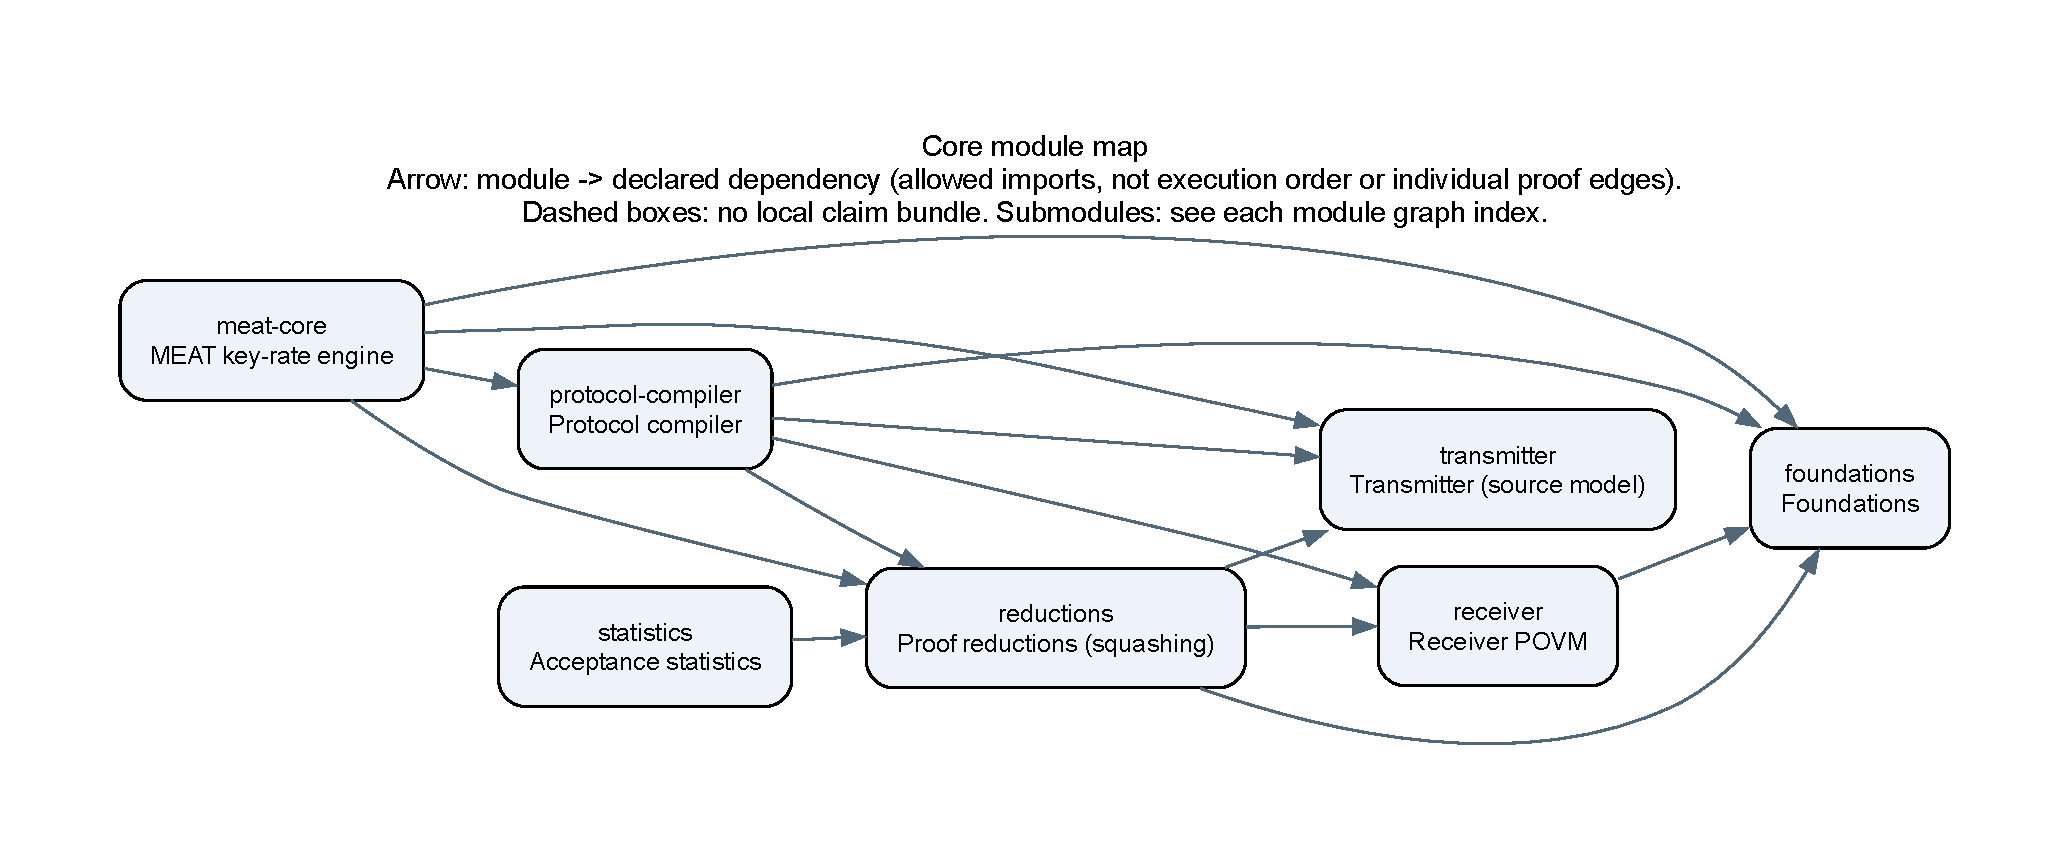
\includegraphics[width=\linewidth]{../module-graph.pdf}


\end{document}
